\documentclass[]{book}
\usepackage{lmodern}
\usepackage{amssymb,amsmath}
\usepackage{ifxetex,ifluatex}
\usepackage{fixltx2e} % provides \textsubscript
\ifnum 0\ifxetex 1\fi\ifluatex 1\fi=0 % if pdftex
  \usepackage[T1]{fontenc}
  \usepackage[utf8]{inputenc}
\else % if luatex or xelatex
  \ifxetex
    \usepackage{mathspec}
  \else
    \usepackage{fontspec}
  \fi
  \defaultfontfeatures{Ligatures=TeX,Scale=MatchLowercase}
\fi
% use upquote if available, for straight quotes in verbatim environments
\IfFileExists{upquote.sty}{\usepackage{upquote}}{}
% use microtype if available
\IfFileExists{microtype.sty}{%
\usepackage{microtype}
\UseMicrotypeSet[protrusion]{basicmath} % disable protrusion for tt fonts
}{}
\usepackage{hyperref}
\hypersetup{unicode=true,
            pdftitle={資料科學與R語言},
            pdfauthor={曾意儒 Yi-Ju Tseng},
            pdfborder={0 0 0},
            breaklinks=true}
\urlstyle{same}  % don't use monospace font for urls
\usepackage{natbib}
\bibliographystyle{apalike}
\usepackage{color}
\usepackage{fancyvrb}
\newcommand{\VerbBar}{|}
\newcommand{\VERB}{\Verb[commandchars=\\\{\}]}
\DefineVerbatimEnvironment{Highlighting}{Verbatim}{commandchars=\\\{\}}
% Add ',fontsize=\small' for more characters per line
\usepackage{framed}
\definecolor{shadecolor}{RGB}{248,248,248}
\newenvironment{Shaded}{\begin{snugshade}}{\end{snugshade}}
\newcommand{\AlertTok}[1]{\textcolor[rgb]{0.94,0.16,0.16}{#1}}
\newcommand{\AnnotationTok}[1]{\textcolor[rgb]{0.56,0.35,0.01}{\textbf{\textit{#1}}}}
\newcommand{\AttributeTok}[1]{\textcolor[rgb]{0.77,0.63,0.00}{#1}}
\newcommand{\BaseNTok}[1]{\textcolor[rgb]{0.00,0.00,0.81}{#1}}
\newcommand{\BuiltInTok}[1]{#1}
\newcommand{\CharTok}[1]{\textcolor[rgb]{0.31,0.60,0.02}{#1}}
\newcommand{\CommentTok}[1]{\textcolor[rgb]{0.56,0.35,0.01}{\textit{#1}}}
\newcommand{\CommentVarTok}[1]{\textcolor[rgb]{0.56,0.35,0.01}{\textbf{\textit{#1}}}}
\newcommand{\ConstantTok}[1]{\textcolor[rgb]{0.00,0.00,0.00}{#1}}
\newcommand{\ControlFlowTok}[1]{\textcolor[rgb]{0.13,0.29,0.53}{\textbf{#1}}}
\newcommand{\DataTypeTok}[1]{\textcolor[rgb]{0.13,0.29,0.53}{#1}}
\newcommand{\DecValTok}[1]{\textcolor[rgb]{0.00,0.00,0.81}{#1}}
\newcommand{\DocumentationTok}[1]{\textcolor[rgb]{0.56,0.35,0.01}{\textbf{\textit{#1}}}}
\newcommand{\ErrorTok}[1]{\textcolor[rgb]{0.64,0.00,0.00}{\textbf{#1}}}
\newcommand{\ExtensionTok}[1]{#1}
\newcommand{\FloatTok}[1]{\textcolor[rgb]{0.00,0.00,0.81}{#1}}
\newcommand{\FunctionTok}[1]{\textcolor[rgb]{0.00,0.00,0.00}{#1}}
\newcommand{\ImportTok}[1]{#1}
\newcommand{\InformationTok}[1]{\textcolor[rgb]{0.56,0.35,0.01}{\textbf{\textit{#1}}}}
\newcommand{\KeywordTok}[1]{\textcolor[rgb]{0.13,0.29,0.53}{\textbf{#1}}}
\newcommand{\NormalTok}[1]{#1}
\newcommand{\OperatorTok}[1]{\textcolor[rgb]{0.81,0.36,0.00}{\textbf{#1}}}
\newcommand{\OtherTok}[1]{\textcolor[rgb]{0.56,0.35,0.01}{#1}}
\newcommand{\PreprocessorTok}[1]{\textcolor[rgb]{0.56,0.35,0.01}{\textit{#1}}}
\newcommand{\RegionMarkerTok}[1]{#1}
\newcommand{\SpecialCharTok}[1]{\textcolor[rgb]{0.00,0.00,0.00}{#1}}
\newcommand{\SpecialStringTok}[1]{\textcolor[rgb]{0.31,0.60,0.02}{#1}}
\newcommand{\StringTok}[1]{\textcolor[rgb]{0.31,0.60,0.02}{#1}}
\newcommand{\VariableTok}[1]{\textcolor[rgb]{0.00,0.00,0.00}{#1}}
\newcommand{\VerbatimStringTok}[1]{\textcolor[rgb]{0.31,0.60,0.02}{#1}}
\newcommand{\WarningTok}[1]{\textcolor[rgb]{0.56,0.35,0.01}{\textbf{\textit{#1}}}}
\usepackage{longtable,booktabs}
\usepackage{graphicx,grffile}
\makeatletter
\def\maxwidth{\ifdim\Gin@nat@width>\linewidth\linewidth\else\Gin@nat@width\fi}
\def\maxheight{\ifdim\Gin@nat@height>\textheight\textheight\else\Gin@nat@height\fi}
\makeatother
% Scale images if necessary, so that they will not overflow the page
% margins by default, and it is still possible to overwrite the defaults
% using explicit options in \includegraphics[width, height, ...]{}
\setkeys{Gin}{width=\maxwidth,height=\maxheight,keepaspectratio}
\IfFileExists{parskip.sty}{%
\usepackage{parskip}
}{% else
\setlength{\parindent}{0pt}
\setlength{\parskip}{6pt plus 2pt minus 1pt}
}
\setlength{\emergencystretch}{3em}  % prevent overfull lines
\providecommand{\tightlist}{%
  \setlength{\itemsep}{0pt}\setlength{\parskip}{0pt}}
\setcounter{secnumdepth}{5}
% Redefines (sub)paragraphs to behave more like sections
\ifx\paragraph\undefined\else
\let\oldparagraph\paragraph
\renewcommand{\paragraph}[1]{\oldparagraph{#1}\mbox{}}
\fi
\ifx\subparagraph\undefined\else
\let\oldsubparagraph\subparagraph
\renewcommand{\subparagraph}[1]{\oldsubparagraph{#1}\mbox{}}
\fi

%%% Use protect on footnotes to avoid problems with footnotes in titles
\let\rmarkdownfootnote\footnote%
\def\footnote{\protect\rmarkdownfootnote}

%%% Change title format to be more compact
\usepackage{titling}

% Create subtitle command for use in maketitle
\providecommand{\subtitle}[1]{
  \posttitle{
    \begin{center}\large#1\end{center}
    }
}

\setlength{\droptitle}{-2em}

  \title{資料科學與R語言}
    \pretitle{\vspace{\droptitle}\centering\huge}
  \posttitle{\par}
    \author{曾意儒 Yi-Ju Tseng}
    \preauthor{\centering\large\emph}
  \postauthor{\par}
      \predate{\centering\large\emph}
  \postdate{\par}
    \date{2019-10-15}


\begin{document}
\maketitle

{
\setcounter{tocdepth}{1}
\tableofcontents
}
\hypertarget{preface}{%
\chapter*{}\label{preface}}
\addcontentsline{toc}{chapter}{}

Placeholder

\hypertarget{intro}{%
\chapter{R語言101}\label{intro}}

Placeholder

\hypertarget{ux4ec0ux9ebcux662frux8a9eux8a00}{%
\section{什麼是R語言}\label{ux4ec0ux9ebcux662frux8a9eux8a00}}

\hypertarget{ux51fdux6578ux4f7fux7528}{%
\section{函數使用}\label{ux51fdux6578ux4f7fux7528}}

\hypertarget{ux8b8aux6578ux8a2dux5b9a}{%
\section{變數設定}\label{ux8b8aux6578ux8a2dux5b9a}}

\hypertarget{ux57f7ux884cux8996ux7a97}{%
\section{執行視窗}\label{ux57f7ux884cux8996ux7a97}}

\hypertarget{DataType}{%
\section{資料型態}\label{DataType}}

\hypertarget{ux6578ux503c-numeric}{%
\subsection{數值 numeric}\label{ux6578ux503c-numeric}}

\hypertarget{ux5b57ux4e32-character}{%
\subsection{字串 character}\label{ux5b57ux4e32-character}}

\hypertarget{ux5e03ux6797ux8b8aux6578-logic}{%
\subsection{布林變數 logic}\label{ux5e03ux6797ux8b8aux6578-logic}}

\hypertarget{ux65e5ux671f-date}{%
\subsection{日期 (Date)}\label{ux65e5ux671f-date}}

\hypertarget{ux57faux672cux904bux7b97ux5b50}{%
\section{基本運算子}\label{ux57faux672cux904bux7b97ux5b50}}

\hypertarget{ux6578ux5b78ux57faux672cux904bux7b97}{%
\subsection{數學基本運算}\label{ux6578ux5b78ux57faux672cux904bux7b97}}

\hypertarget{ux908fux8f2fux904bux7b97}{%
\subsection{邏輯運算}\label{ux908fux8f2fux904bux7b97}}

\hypertarget{ux932fux8aa4ux8a0aux606f}{%
\section{錯誤訊息}\label{ux932fux8aa4ux8a0aux606f}}

\hypertarget{help}{%
\section{Help}\label{help}}

\hypertarget{RDataStructure}{%
\chapter{R 資料結構}\label{RDataStructure}}

Placeholder

\hypertarget{ux5411ux91cf-vector}{%
\section{向量 vector}\label{ux5411ux91cf-vector}}

\hypertarget{ux5febux901fux7522ux751fux5411ux91cfux51fdux6578}{%
\subsection{快速產生向量函數}\label{ux5febux901fux7522ux751fux5411ux91cfux51fdux6578}}

\hypertarget{ux5411ux91cfux904bux7b97}{%
\subsection{向量運算}\label{ux5411ux91cfux904bux7b97}}

\hypertarget{ux56e0ux5b50-factor}{%
\section{因子 factor}\label{ux56e0ux5b50-factor}}

\hypertarget{ux5217ux8868-list}{%
\section{列表 list}\label{ux5217ux8868-list}}

\hypertarget{ux5217ux8868ux8cc7ux6599ux64f7ux53d6}{%
\subsection{列表資料擷取}\label{ux5217ux8868ux8cc7ux6599ux64f7ux53d6}}

\hypertarget{ux5217ux8868ux8cc7ux6599ux7de8ux8f2fux8a2dux5b9a}{%
\subsection{列表資料編輯設定}\label{ux5217ux8868ux8cc7ux6599ux7de8ux8f2fux8a2dux5b9a}}

\hypertarget{ux77e9ux9663-matrix}{%
\section{矩陣 matrix}\label{ux77e9ux9663-matrix}}

\hypertarget{ux8cc7ux6599ux6846-data.frame}{%
\section{資料框 data.frame}\label{ux8cc7ux6599ux6846-data.frame}}

\hypertarget{ux8cc7ux6599ux8868-data.table}{%
\section{資料表 data.table}\label{ux8cc7ux6599ux8868-data.table}}

\hypertarget{ux8cc7ux6599ux5c6cux6027ux67e5ux8a62ux51fdux6578}{%
\section{資料屬性查詢函數}\label{ux8cc7ux6599ux5c6cux6027ux67e5ux8a62ux51fdux6578}}

\hypertarget{controlstructure}{%
\chapter{控制流程}\label{controlstructure}}

Placeholder

\hypertarget{ux689dux4ef6ux5224ux65b7}{%
\section{條件判斷}\label{ux689dux4ef6ux5224ux65b7}}

\hypertarget{if-elseux6558ux8ff0}{%
\subsection{if-else敘述}\label{if-elseux6558ux8ff0}}

\hypertarget{if-else-if-else}{%
\subsection{if-else if-else}\label{if-else-if-else}}

\hypertarget{function}{%
\chapter{函數}\label{function}}

Placeholder

\hypertarget{io}{%
\chapter{資料讀取與匯出}\label{io}}

Placeholder

\hypertarget{ux7d14ux6587ux5b57ux8cc7ux6599-ux7121ux5206ux9694}{%
\subsection{純文字資料 (無分隔)}\label{ux7d14ux6587ux5b57ux8cc7ux6599-ux7121ux5206ux9694}}

\hypertarget{ux5176ux4ed6ux8b80ux6a94ux6ce8ux610fux4e8bux9805}{%
\subsection{其他讀檔注意事項}\label{ux5176ux4ed6ux8b80ux6a94ux6ce8ux610fux4e8bux9805}}

\hypertarget{open-data}{%
\subsection{Open Data}\label{open-data}}

\hypertarget{api}{%
\subsection{API (Application programming interfaces)}\label{api}}

\hypertarget{xml}{%
\subsection{XML 可延伸標記式語言}\label{xml}}

\hypertarget{ux7db2ux9801ux722cux87f2-webscraping}{%
\subsection{網頁爬蟲 Webscraping}\label{ux7db2ux9801ux722cux87f2-webscraping}}

\hypertarget{facebookux8cc7ux6599ux64f7ux53d6}{%
\section{Facebook資料擷取}\label{facebookux8cc7ux6599ux64f7ux53d6}}

\hypertarget{graph-api-in-r}{%
\subsection{Graph API in R}\label{graph-api-in-r}}

\hypertarget{rfacebook-package}{%
\subsection{Rfacebook package}\label{rfacebook-package}}

\hypertarget{manipulation}{%
\chapter{資料處理與清洗}\label{manipulation}}

Placeholder

\hypertarget{tidy-data}{%
\section{Tidy Data}\label{tidy-data}}

\hypertarget{ux8cc7ux6599ux578bux5225ux8f49ux63dbux8655ux7406}{%
\section{資料型別轉換處理}\label{ux8cc7ux6599ux578bux5225ux8f49ux63dbux8655ux7406}}

\hypertarget{ux6587ux5b57ux5b57ux4e32ux8655ux7406}{%
\section{文字字串處理}\label{ux6587ux5b57ux5b57ux4e32ux8655ux7406}}

\hypertarget{ux57faux672cux8655ux7406}{%
\subsection{基本處理}\label{ux57faux672cux8655ux7406}}

\hypertarget{ux641cux5c0bux5b57ux4e32}{%
\subsection{搜尋字串}\label{ux641cux5c0bux5b57ux4e32}}

\hypertarget{ux6b63ux898fux8868ux793aux5f0f-regular-expression}{%
\subsection{正規表示式 (Regular Expression)}\label{ux6b63ux898fux8868ux793aux5f0f-regular-expression}}

\hypertarget{ux9003ux812bux5b57ux5143}{%
\subsubsection{逃脫字元}\label{ux9003ux812bux5b57ux5143}}

\hypertarget{ux8868ux793aux6578ux91cfux7684ux8a9eux6cd5}{%
\subsubsection{表示數量的語法}\label{ux8868ux793aux6578ux91cfux7684ux8a9eux6cd5}}

\hypertarget{ux8868ux793aux4f4dux7f6eux7684ux8a9eux6cd5}{%
\subsubsection{表示位置的語法}\label{ux8868ux793aux4f4dux7f6eux7684ux8a9eux6cd5}}

\hypertarget{ux904bux7b97ux5b50}{%
\subsubsection{運算子}\label{ux904bux7b97ux5b50}}

\hypertarget{ux7279ux6b8aux7b26ux865f}{%
\subsubsection{特殊符號}\label{ux7279ux6b8aux7b26ux865f}}

\hypertarget{ux53c3ux8003ux8cc7ux6599}{%
\subsubsection{參考資料}\label{ux53c3ux8003ux8cc7ux6599}}

\hypertarget{ux8f09ux5165ux8cc7ux6599}{%
\subsection{載入資料}\label{ux8f09ux5165ux8cc7ux6599}}

\hypertarget{eda}{%
\chapter{探索式資料分析}\label{eda}}

Placeholder

\hypertarget{ux4ec0ux9ebcux662fux63a2ux7d22ux5f0fux8cc7ux6599ux5206ux6790}{%
\section{什麼是探索式資料分析}\label{ux4ec0ux9ebcux662fux63a2ux7d22ux5f0fux8cc7ux6599ux5206ux6790}}

\hypertarget{datatable}{%
\section{data.table}\label{datatable}}

\hypertarget{i-ux89c0ux5bdfux503cux7be9ux9078ux908fux8f2f}{%
\subsection{i 觀察值篩選邏輯}\label{i-ux89c0ux5bdfux503cux7be9ux9078ux908fux8f2f}}

\hypertarget{j-ux6b04ux4f4dux9078ux64c7ux904bux7b97}{%
\subsection{j 欄位選擇運算}\label{j-ux6b04ux4f4dux9078ux64c7ux904bux7b97}}

\hypertarget{by-ux5206ux7d44ux4f9dux64da}{%
\subsection{by 分組依據}\label{by-ux5206ux7d44ux4f9dux64da}}

\hypertarget{ux53c3ux8003ux6587ux4ef6ux8207ux8cc7ux6e90}{%
\subsection{參考文件與資源}\label{ux53c3ux8003ux6587ux4ef6ux8207ux8cc7ux6e90}}

\hypertarget{dplyr}{%
\section{dplyr}\label{dplyr}}

\hypertarget{select}{%
\subsection{select()}\label{select}}

\hypertarget{filter}{%
\subsection{filter()}\label{filter}}

\hypertarget{mutate}{%
\subsection{mutate()}\label{mutate}}

\hypertarget{summarise}{%
\subsection{summarise()}\label{summarise}}

\hypertarget{group_by}{%
\subsection{group\_by()}\label{group_by}}

\hypertarget{arrange}{%
\subsection{arrange()}\label{arrange}}

\hypertarget{rename}{%
\subsection{rename()}\label{rename}}

\hypertarget{ux53c3ux8003ux6587ux4ef6ux8207ux8cc7ux6e90-1}{%
\subsection{參考文件與資源}\label{ux53c3ux8003ux6587ux4ef6ux8207ux8cc7ux6e90-1}}

\hypertarget{vis}{%
\chapter{資料視覺化}\label{vis}}

Placeholder

\hypertarget{ux8cc7ux6599ux8996ux89baux5316ux7684ux76eeux7684}{%
\section{資料視覺化的目的}\label{ux8cc7ux6599ux8996ux89baux5316ux7684ux76eeux7684}}

\hypertarget{ggplot2ux7c21ux4ecb}{%
\section{ggplot2簡介}\label{ggplot2ux7c21ux4ecb}}

\hypertarget{qplot}{%
\subsection{qplot()}\label{qplot}}

\hypertarget{ggplot}{%
\subsection{ggplot()}\label{ggplot}}

\hypertarget{ggplot2ux5730ux5716}{%
\section{ggplot2+地圖}\label{ggplot2ux5730ux5716}}

\hypertarget{choropleth-mapux9762ux91cfux5716}{%
\subsection{Choropleth map面量圖}\label{choropleth-mapux9762ux91cfux5716}}

\hypertarget{ggmap}{%
\subsection{ggmap()}\label{ggmap}}

\hypertarget{taiwanux7684ux9762ux91cfux5716}{%
\section{Taiwan的面量圖}\label{taiwanux7684ux9762ux91cfux5716}}

\hypertarget{ggmapux9762ux91cfux5716}{%
\subsection{ggmap+面量圖}\label{ggmapux9762ux91cfux5716}}

\hypertarget{treemap}{%
\section{Treemap}\label{treemap}}

\hypertarget{ux53c3ux8003ux6587ux4ef6ux8207ux8cc7ux6e90-2}{%
\section{參考文件與資源}\label{ux53c3ux8003ux6587ux4ef6ux8207ux8cc7ux6e90-2}}

\hypertarget{InteractiveGraphics}{%
\chapter{互動式資料呈現}\label{InteractiveGraphics}}

Placeholder

\hypertarget{ggvis}{%
\section{ggvis}\label{ggvis}}

\hypertarget{plot.ly}{%
\section{Plot.ly}\label{plot.ly}}

\hypertarget{shinyux7c21ux4ecb}{%
\section{Shiny簡介}\label{shinyux7c21ux4ecb}}

\hypertarget{datamining}{%
\chapter{資料探勘}\label{datamining}}

\textbf{撰寫中}

\hypertarget{ux4ec0ux9ebcux662fux8cc7ux6599ux63a2ux52d8}{%
\section{什麼是資料探勘}\label{ux4ec0ux9ebcux662fux8cc7ux6599ux63a2ux52d8}}

\textbf{資料探勘(Data mining)}是用人工智慧、機器學習、統計學的交叉方法,在相對較大型的資料集中發現模式的計算過程。使用資料探勘技術可以建立從\textbf{輸入資料}學習新資訊,變成智慧的\textbf{演算法}或\textbf{資料模式},用來\textbf{預測事件}或\textbf{協助決策}。所以,當資料太\texttt{少}或\texttt{太髒}的時候,資料探勘的效力會被影響。

資料探勘要派上用場,必須有以下條件:

\begin{itemize}
\tightlist
\item
  有一些模式/模型可\texttt{學}
\item
  很難定義這些模式/模型
\item
  有資料可\texttt{學}這些模式/模型
\end{itemize}

資料探勘的應用範例如下:

\begin{itemize}
\tightlist
\item
  天氣預測
\item
  搜尋建議、購物建議
\item
  股市預測
\item
  臉部辨識、指紋辨識
\item
  垃圾郵件標記
\item
  尿布啤酒
\end{itemize}

資料探勘可分為\textbf{監督式}學習與\textbf{非監督式}學習,監督式學習的特點是訓練資料中有\textbf{正確答案},由輸入物件和預期輸出所組成,而演算法可以由訓練資料中學到或建立一個模式,並依此模式推測新的實例;非監督式學習則不用提供\textbf{正確答案},也就是不需要人力來輸入標籤,單純利用訓練資料的特性,將資料分群分組。

此兩種學習可解決不同的問題,條列如下:

\begin{itemize}
\tightlist
\item
  Supervised learning 監督式學習

  \begin{itemize}
  \tightlist
  \item
    Regression 迴歸:真實的'值'(股票、氣溫)
  \item
    Classification 分類:分兩類(P/N, Yes/No, M/F, Sick/Not sick)/分多類 (A/B/C/D)
  \end{itemize}
\item
  Unsupervised learning 非監督式學習

  \begin{itemize}
  \tightlist
  \item
    Clustering 分群
  \item
    Association Rules 關聯式規則
  \end{itemize}
\end{itemize}

在\textbf{監督式}學習中常見的資料探勘演算法如下:

\begin{itemize}
\tightlist
\item
  Linear Regression 線性迴歸
\item
  Logistic Regression 羅吉斯迴歸、邏輯迴歸
\item
  Support Vector Machines 支持向量機
\item
  Decision Trees 決策樹
\item
  K-Nearest Neighbor
\item
  Neural Networks 神經網路
\item
  Deep Learning 深度學習
\end{itemize}

在\textbf{非監督式}學習中常見的資料探勘演算法如下:

\begin{itemize}
\tightlist
\item
  Hierarchical clustering 階層式分群
\item
  K-means clustering
\item
  Neural Networks 神經網路
\item
  Deep Learning 深度學習
\end{itemize}

以下介紹在R中使用各類演算法的方法

\hypertarget{regression-ux8ff4ux6b78}{%
\section{Regression 迴歸}\label{regression-ux8ff4ux6b78}}

Regression Analysis 迴歸分析主要用在了解兩個或多個變數間\texttt{是否相關}、\texttt{相關方向與強度},並建立\texttt{數學模型}以便觀察特定變數來預測研究者感興趣的變數,常見的迴歸分析演算法包括:

\begin{itemize}
\tightlist
\item
  Linear Regression 線性迴歸
\item
  Logistic Regression 羅吉斯迴歸、邏輯迴歸
\end{itemize}

\hypertarget{linear-regression-ux7ddaux6027ux8ff4ux6b78}{%
\subsection{Linear Regression 線性迴歸}\label{linear-regression-ux7ddaux6027ux8ff4ux6b78}}

首先,嘗試將Linear Regression 線性迴歸用在NBA的資料看看,做NBA\texttt{得分}與\texttt{上場分鐘數}的線性迴歸觀察

\begin{Shaded}
\begin{Highlighting}[]
\CommentTok{#讀入SportsAnalytics package}
\KeywordTok{library}\NormalTok{(SportsAnalytics)}
\CommentTok{#擷取2015-2016年球季球員資料}
\NormalTok{NBA1516<-}\KeywordTok{fetch_NBAPlayerStatistics}\NormalTok{(}\StringTok{"15-16"}\NormalTok{)}
\end{Highlighting}
\end{Shaded}

\begin{Shaded}
\begin{Highlighting}[]
\KeywordTok{library}\NormalTok{(ggplot2)}
\KeywordTok{ggplot}\NormalTok{(NBA1516,}\KeywordTok{aes}\NormalTok{(}\DataTypeTok{x=}\NormalTok{TotalMinutesPlayed,}\DataTypeTok{y=}\NormalTok{TotalPoints))}\OperatorTok{+}
\StringTok{    }\KeywordTok{geom_point}\NormalTok{()}\OperatorTok{+}\KeywordTok{geom_smooth}\NormalTok{(}\DataTypeTok{method =} \StringTok{"glm"}\NormalTok{)}
\end{Highlighting}
\end{Shaded}

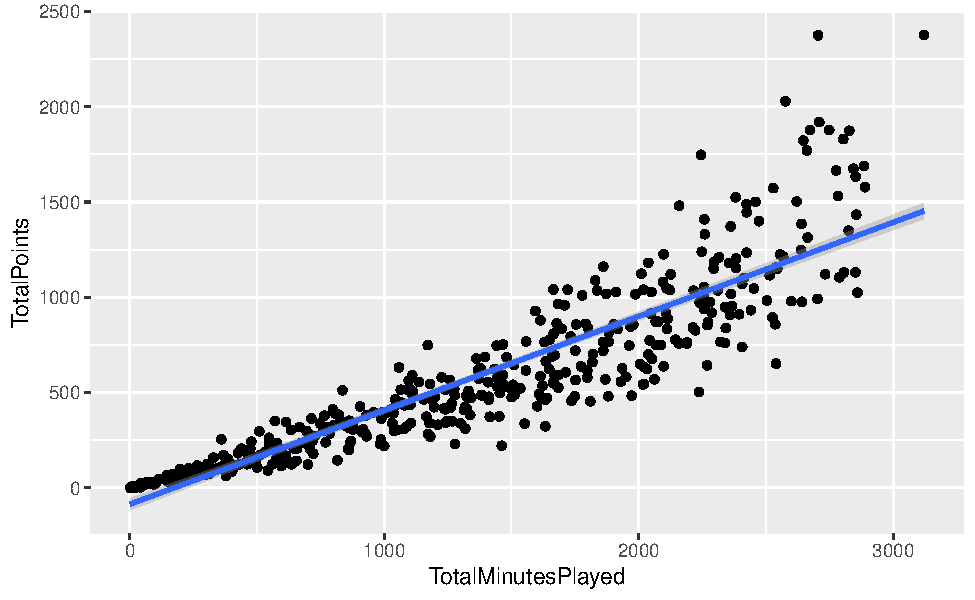
\includegraphics{DataAnalyticsWithR_files/figure-latex/linear2-1.pdf}

在R中,最基本的簡單線性迴歸分析為\texttt{lm()},使用方法為\texttt{lm(formula,data=資料名稱)},搭配formula使用,formula的撰寫方法為:依變項\textasciitilde 自變項1+自變項2+\ldots.

\begin{Shaded}
\begin{Highlighting}[]
\KeywordTok{lm}\NormalTok{(TotalPoints}\OperatorTok{~}\NormalTok{TotalMinutesPlayed,}\DataTypeTok{data =}\NormalTok{NBA1516)}
\end{Highlighting}
\end{Shaded}

\begin{verbatim}
## 
## Call:
## lm(formula = TotalPoints ~ TotalMinutesPlayed, data = NBA1516)
## 
## Coefficients:
##        (Intercept)  TotalMinutesPlayed  
##           -85.9071              0.4931
\end{verbatim}

由此可知總得分數TotalPoints等於\texttt{0.4931} * 總出場分鐘數 \texttt{-85.9071}

TotalPoints = \texttt{0.4931} * TotalMinutesPlayed \texttt{-85.9071}

更被廣泛使用的是廣義線性迴歸模型generalized linear models (glm),函數為\texttt{glm()},使用方法與\texttt{lm()}類似,包括了線性迴歸模型和邏輯迴歸模型。
如果需要修改預設模型,可設定family參數:

\begin{verbatim}
- `family="gaussian"` 線性模型模型
- `family="binomial"` 邏輯迴歸模型
- `family="poisson"` 卜瓦松迴歸模型
\end{verbatim}

Gaussian distribution高斯函數是\texttt{常態分布}的密度函數

Binomial distribution二項分布是\texttt{n個獨立的是/非試驗中成功的次數}的離散機率分布

Poisson distribution\texttt{次數}分佈:

\begin{itemize}
\tightlist
\item
  某一服務設施在一定時間內受到的服務請求的次數
\item
  公車站的候客人數
\item
  機器故障數
\item
  自然災害發生的次數
\item
  DNA序列的變異數\ldots..
\end{itemize}

以下為使用多變量線性迴歸來分析\texttt{得分}與\texttt{上場分鐘數}和\texttt{兩分球出手數}的關係範例

\begin{Shaded}
\begin{Highlighting}[]
\CommentTok{# e+01: 10^1 / e-04: 10^(-4)}
\KeywordTok{glm}\NormalTok{(TotalPoints}\OperatorTok{~}\NormalTok{TotalMinutesPlayed}\OperatorTok{+}\NormalTok{FieldGoalsAttempted,}
    \DataTypeTok{data =}\NormalTok{NBA1516)}
\end{Highlighting}
\end{Shaded}

\begin{verbatim}
## 
## Call:  glm(formula = TotalPoints ~ TotalMinutesPlayed + FieldGoalsAttempted, 
##     data = NBA1516)
## 
## Coefficients:
##         (Intercept)   TotalMinutesPlayed  FieldGoalsAttempted  
##          -1.799e+01           -2.347e-04            1.256e+00  
## 
## Degrees of Freedom: 475 Total (i.e. Null);  473 Residual
## Null Deviance:       99360000 
## Residual Deviance: 2160000   AIC: 5367
\end{verbatim}

由此可知總得分數等於\texttt{-0.0002347} * 總出場分鐘數 + \texttt{1.255794} * 兩分球出手數 \texttt{-17.99}
TotalPoints = \texttt{-0.0002347} * TotalMinutesPlayed + \texttt{1.255794} * FieldGoalsAttempted \texttt{-17.99}

如需使用多變量線性迴歸來分析\texttt{得分}與\texttt{上場分鐘數}和\texttt{兩分球出手數}和\texttt{守備位置}的關係,可修改formula

\begin{Shaded}
\begin{Highlighting}[]
\KeywordTok{glm}\NormalTok{(TotalPoints}\OperatorTok{~}\NormalTok{TotalMinutesPlayed}\OperatorTok{+}\NormalTok{FieldGoalsAttempted}\OperatorTok{+}\NormalTok{Position,}
    \DataTypeTok{data =}\NormalTok{NBA1516)}
\end{Highlighting}
\end{Shaded}

\begin{verbatim}
## 
## Call:  glm(formula = TotalPoints ~ TotalMinutesPlayed + FieldGoalsAttempted + 
##     Position, data = NBA1516)
## 
## Coefficients:
##         (Intercept)   TotalMinutesPlayed  FieldGoalsAttempted  
##           22.852223            -0.006537             1.275721  
##          PositionPF           PositionPG           PositionSF  
##          -39.416327           -65.034646           -38.522299  
##          PositionSG  
##          -52.175144  
## 
## Degrees of Freedom: 474 Total (i.e. Null);  468 Residual
##   (1 observation deleted due to missingness)
## Null Deviance:       99080000 
## Residual Deviance: 1975000   AIC: 5322
\end{verbatim}

\begin{Shaded}
\begin{Highlighting}[]
\CommentTok{# e+01: 10^1 / e-04: 10^(-4)}
\end{Highlighting}
\end{Shaded}

由此可知總得分數TotalPoints和\texttt{上場分鐘數}和\texttt{兩分球出手數}和\texttt{守備位置}的關係為:
TotalPoints = \texttt{-0.0065} * TotalMinutesPlayed + \texttt{1.28} \emph{FieldGoalsAttempted \texttt{+22.85} + \texttt{22.85} } PositionPF + \texttt{-65.03} * PositionPG + \texttt{-38.52} * PositionSF + \texttt{-52.18} * PositionSG

由上述結果可發現,\texttt{守備位置}的變項被轉為\textbf{虛擬變項 Dummy Variable}:PositionPF、PositionPG、PositionSF、PositionSG,如果是控球後衛(PG),會得到:

\begin{itemize}
\tightlist
\item
  PositionPF=0
\item
  PositionPG=1
\item
  PositionSF=0
\item
  PositionSG=0
\end{itemize}

可能有人會問,那中鋒去哪了?其實中鋒被當作基準項,也就是當守備位置是中鋒(C)時,會得到:

\begin{itemize}
\tightlist
\item
  PositionPF=0
\item
  PositionPG=0
\item
  PositionSF=0
\item
  PositionSG=0
\end{itemize}

總結以上,多變量線性迴歸分析有下列特色:

\begin{itemize}
\tightlist
\item
  假設:各變數相互獨立!
\item
  若自變項X是類別變項,需要建立\texttt{虛擬變項}
\item
  在R裡,\texttt{類別變項}請記得轉成factor,R會自動建立\texttt{虛擬變項}
\item
  用在\texttt{依變數為連續變數},\texttt{自變數為連續變數或虛擬變數}的場合
\end{itemize}

\hypertarget{logistic-regression-ux7f85ux5409ux65afux8ff4ux6b78}{%
\subsection{Logistic Regression 羅吉斯迴歸}\label{logistic-regression-ux7f85ux5409ux65afux8ff4ux6b78}}

Logistic Regression 羅吉斯迴歸常用在\texttt{依變數為二元變數(非0即1)}的場合,如:
- 生病/沒生病
- 錄取/不錄取
- \texttt{family="binomial"} 邏輯迴歸模型

以分數資料為例,分析為什麼錄取/不錄取?

\begin{Shaded}
\begin{Highlighting}[]
\NormalTok{mydata <-}\StringTok{ }\KeywordTok{read.csv}\NormalTok{(}\StringTok{"https://raw.githubusercontent.com/CGUIM-BigDataAnalysis/BigDataCGUIM/master/binary.csv"}\NormalTok{)}
\end{Highlighting}
\end{Shaded}

\begin{Shaded}
\begin{Highlighting}[]
\CommentTok{# GRE:某考試成績, GPA:在校平均成績, rank:學校聲望}
\KeywordTok{head}\NormalTok{(mydata)}
\end{Highlighting}
\end{Shaded}

\begin{tabular}{r|r|r|r}
\hline
admit & gre & gpa & rank\\
\hline
0 & 380 & 3.61 & 3\\
\hline
1 & 660 & 3.67 & 3\\
\hline
1 & 800 & 4.00 & 1\\
\hline
1 & 640 & 3.19 & 4\\
\hline
0 & 520 & 2.93 & 4\\
\hline
1 & 760 & 3.00 & 2\\
\hline
\end{tabular}

\begin{Shaded}
\begin{Highlighting}[]
\NormalTok{mydata}\OperatorTok{$}\NormalTok{rank <-}\StringTok{ }\KeywordTok{factor}\NormalTok{(mydata}\OperatorTok{$}\NormalTok{rank)}
\NormalTok{mylogit <-}\StringTok{ }\KeywordTok{glm}\NormalTok{(admit }\OperatorTok{~}\StringTok{ }\NormalTok{gre }\OperatorTok{+}\StringTok{ }\NormalTok{gpa }\OperatorTok{+}\StringTok{ }\NormalTok{rank,}
               \DataTypeTok{data =}\NormalTok{ mydata, }\DataTypeTok{family =} \StringTok{"binomial"}\NormalTok{)}
\NormalTok{sum<-}\KeywordTok{summary}\NormalTok{(mylogit)}
\NormalTok{sum}\OperatorTok{$}\NormalTok{coefficients}
\end{Highlighting}
\end{Shaded}

\begin{verbatim}
##                 Estimate  Std. Error   z value     Pr(>|z|)
## (Intercept) -3.989979073 1.139950936 -3.500132 0.0004650273
## gre          0.002264426 0.001093998  2.069864 0.0384651284
## gpa          0.804037549 0.331819298  2.423119 0.0153878974
## rank2       -0.675442928 0.316489661 -2.134171 0.0328288188
## rank3       -1.340203916 0.345306418 -3.881202 0.0001039415
## rank4       -1.551463677 0.417831633 -3.713131 0.0002047107
\end{verbatim}

\hypertarget{ux6700ux4f73ux6a21ux578bux7be9ux9078}{%
\subsection{最佳模型篩選}\label{ux6700ux4f73ux6a21ux578bux7be9ux9078}}

到底該用哪個模型來預測,會得到最準確的結果?在迴歸模型中,常用的判斷準則包括:

\begin{itemize}
\tightlist
\item
  Akaike's Information Criterion (AIC)
\item
  Bayesian Information Criterion (BIC)
\end{itemize}

AIC和BIC都是數值越小越好,以下建立三個模型,並比較其AIC,

\begin{Shaded}
\begin{Highlighting}[]
\NormalTok{OneVar<-}\KeywordTok{glm}\NormalTok{(TotalPoints}\OperatorTok{~}\NormalTok{TotalMinutesPlayed,}\DataTypeTok{data =}\NormalTok{NBA1516)}
\NormalTok{TwoVar<-}\KeywordTok{glm}\NormalTok{(TotalPoints}\OperatorTok{~}\NormalTok{TotalMinutesPlayed}\OperatorTok{+}\NormalTok{FieldGoalsAttempted,}
            \DataTypeTok{data =}\NormalTok{NBA1516)}
\NormalTok{ThreeVar<-}\KeywordTok{glm}\NormalTok{(TotalPoints}\OperatorTok{~}\NormalTok{TotalMinutesPlayed}\OperatorTok{+}\NormalTok{FieldGoalsAttempted}\OperatorTok{+}\NormalTok{Position,}
              \DataTypeTok{data =}\NormalTok{NBA1516)}
\KeywordTok{c}\NormalTok{(OneVar}\OperatorTok{$}\NormalTok{aic,TwoVar}\OperatorTok{$}\NormalTok{aic,ThreeVar}\OperatorTok{$}\NormalTok{aic)}
\end{Highlighting}
\end{Shaded}

\begin{verbatim}
## [1] 6338.913 5366.763 5321.972
\end{verbatim}

在建立迴歸模型時,常會遇到到底該放多少參數?所有參數都有用嗎?這類的問題,我們可以藉由觀察coefficients來判斷參數在模型中的``實用程度''

\begin{Shaded}
\begin{Highlighting}[]
\NormalTok{sum2<-}\KeywordTok{summary}\NormalTok{(TwoVar)}
\NormalTok{sum2}\OperatorTok{$}\NormalTok{coefficients}
\end{Highlighting}
\end{Shaded}

\begin{verbatim}
##                          Estimate  Std. Error     t value      Pr(>|t|)
## (Intercept)         -1.798855e+01 5.659758251 -3.17832538  1.578333e-03
## TotalMinutesPlayed  -2.347183e-04 0.009474631 -0.02477334  9.802462e-01
## FieldGoalsAttempted  1.255794e+00 0.022239494 56.46682752 2.474028e-212
\end{verbatim}

\begin{Shaded}
\begin{Highlighting}[]
\NormalTok{sum3<-}\KeywordTok{summary}\NormalTok{(ThreeVar)}
\NormalTok{sum3}\OperatorTok{$}\NormalTok{coefficients}
\end{Highlighting}
\end{Shaded}

\begin{verbatim}
##                          Estimate   Std. Error    t value      Pr(>|t|)
## (Intercept)          22.852222668  9.014714391  2.5349913  1.156964e-02
## TotalMinutesPlayed   -0.006536874  0.009199968 -0.7105322  4.777281e-01
## FieldGoalsAttempted   1.275721212  0.021647176 58.9324535 1.144607e-218
## PositionPF          -39.416326742  9.936541704 -3.9668053  8.425605e-05
## PositionPG          -65.034646215 10.269250388 -6.3329497  5.648565e-10
## PositionSF          -38.522298887 10.488170409 -3.6729284  2.674727e-04
## PositionSG          -52.175143670  9.985331185 -5.2251791  2.625062e-07
\end{verbatim}

\hypertarget{decision-trees-ux6c7aux7b56ux6a39}{%
\section{Decision Trees 決策樹}\label{decision-trees-ux6c7aux7b56ux6a39}}

決策樹是在\texttt{樹狀目錄}中建立一系列分割,以建立模型。這些分割會表示成\texttt{「節點」(Node)}。每次發現輸入資料行與可預測資料行有明顯地相互關聯時,此演算法就會在模型中加入一個\texttt{節點}。演算法決定分岔的方式不同,視它預測連續資料行或分隔資料行而定。

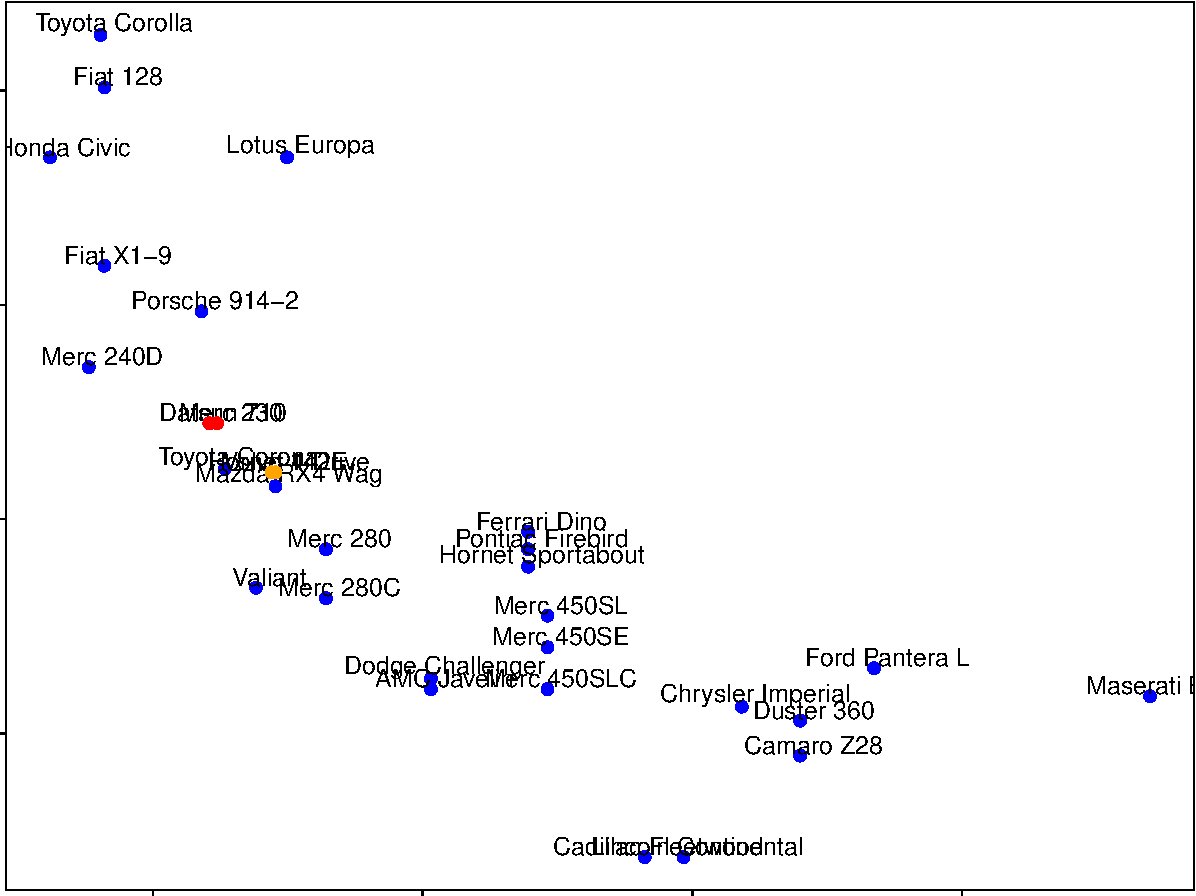
\includegraphics{DataAnalyticsWithR_files/figure-latex/unnamed-chunk-3-1.pdf}

以下介紹常見的Classification And Regression Tree (CART),使用前須先安裝\texttt{rpart} packages \citep{R-rpart}

\begin{Shaded}
\begin{Highlighting}[]
\KeywordTok{install.packages}\NormalTok{(}\StringTok{"rpart"}\NormalTok{)}
\end{Highlighting}
\end{Shaded}

以前述NBA資料為例,嘗試用用籃板/三分/助攻/抄截數據來判斷守備位置,建立決策樹的函數為\texttt{rpart()},使用方式為\texttt{rpart(formula,\ data)}

\begin{Shaded}
\begin{Highlighting}[]
\KeywordTok{library}\NormalTok{(rpart)}
\NormalTok{DT<-}\KeywordTok{rpart}\NormalTok{(Position}\OperatorTok{~}\NormalTok{Blocks}\OperatorTok{+}\NormalTok{ThreesMade}\OperatorTok{+}\NormalTok{Assists}\OperatorTok{+}\NormalTok{Steals,}\DataTypeTok{data=}\NormalTok{NBA1516)}
\NormalTok{DT}
\end{Highlighting}
\end{Shaded}

\begin{verbatim}
## n=475 (1 observation deleted due to missingness)
## 
## node), split, n, loss, yval, (yprob)
##       * denotes terminal node
## 
##   1) root 475 364 PF (0.15 0.23 0.21 0.18 0.23)  
##     2) ThreesMade< 2.5 132  74 C (0.44 0.35 0.098 0.053 0.061)  
##       4) Blocks>=4.5 89  37 C (0.58 0.38 0.011 0.011 0.011) *
##       5) Blocks< 4.5 43  31 PF (0.14 0.28 0.28 0.14 0.16)  
##        10) Steals< 2.5 29  19 PF (0.17 0.34 0.14 0.21 0.14) *
##        11) Steals>=2.5 14   6 PG (0.071 0.14 0.57 0 0.21) *
##     3) ThreesMade>=2.5 343 242 SG (0.035 0.19 0.25 0.23 0.29)  
##       6) Assists>=170.5 96  39 PG (0.031 0.052 0.59 0.15 0.18) *
##       7) Assists< 170.5 247 163 SG (0.036 0.24 0.12 0.26 0.34)  
##        14) Blocks>=20.5 80  42 PF (0.062 0.48 0 0.26 0.2)  
##          28) Steals< 59.5 58  21 PF (0.069 0.64 0 0.14 0.16) *
##          29) Steals>=59.5 22   9 SF (0.045 0.045 0 0.59 0.32) *
##        15) Blocks< 20.5 167  99 SG (0.024 0.13 0.17 0.26 0.41)  
##          30) Assists< 81.5 110  68 SG (0.027 0.18 0.091 0.32 0.38)  
##            60) Blocks>=4.5 63  39 SF (0.032 0.29 0.016 0.38 0.29)  
##             120) ThreesMade< 13.5 19   9 PF (0.11 0.53 0 0.26 0.11) *
##             121) ThreesMade>=13.5 44  25 SF (0 0.18 0.023 0.43 0.36)  
##               242) Blocks< 9.5 17   7 SF (0 0.18 0.059 0.59 0.18) *
##               243) Blocks>=9.5 27  14 SG (0 0.19 0 0.33 0.48) *
##            61) Blocks< 4.5 47  23 SG (0.021 0.043 0.19 0.23 0.51) *
##          31) Assists>=81.5 57  31 SG (0.018 0.035 0.33 0.16 0.46)  
##            62) ThreesMade< 37 17   5 PG (0 0.12 0.71 0.059 0.12) *
##            63) ThreesMade>=37 40  16 SG (0.025 0 0.17 0.2 0.6) *
\end{verbatim}

\begin{Shaded}
\begin{Highlighting}[]
\CommentTok{#控球後衛(PG)、得分後衛(SG)、小前鋒(SF)、大前鋒(PF)和中鋒(C)}
\end{Highlighting}
\end{Shaded}

\begin{Shaded}
\begin{Highlighting}[]
\KeywordTok{par}\NormalTok{(}\DataTypeTok{mfrow=}\KeywordTok{c}\NormalTok{(}\DecValTok{1}\NormalTok{,}\DecValTok{1}\NormalTok{), }\DataTypeTok{mar =} \KeywordTok{rep}\NormalTok{(}\DecValTok{1}\NormalTok{,}\DecValTok{4}\NormalTok{)) }\CommentTok{#下,左,上,右}
\KeywordTok{plot}\NormalTok{(DT)}
\KeywordTok{text}\NormalTok{(DT, }\DataTypeTok{use.n=}\NormalTok{F, }\DataTypeTok{all=}\NormalTok{F, }\DataTypeTok{cex=}\DecValTok{1}\NormalTok{)}
\end{Highlighting}
\end{Shaded}

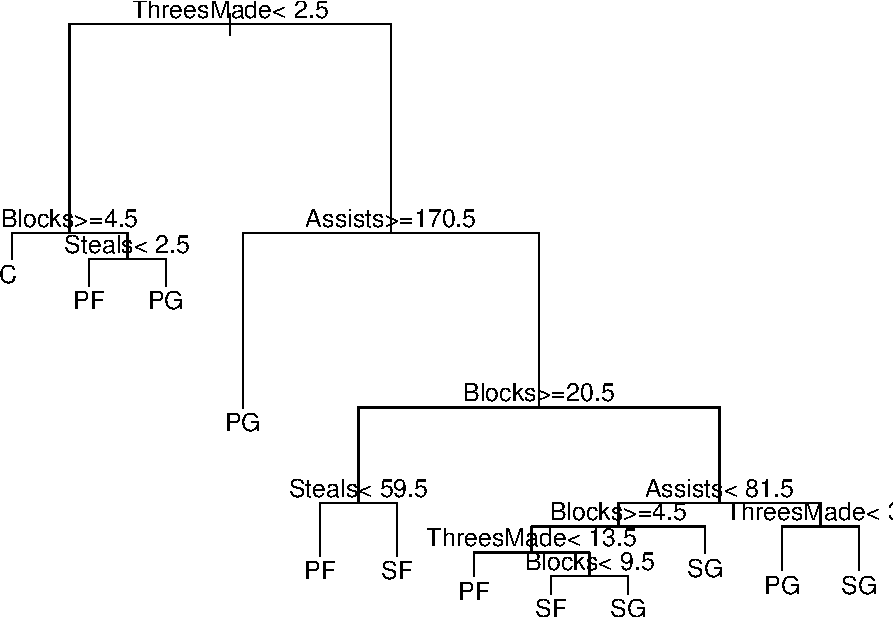
\includegraphics{DataAnalyticsWithR_files/figure-latex/rpart3-1.pdf}

\begin{Shaded}
\begin{Highlighting}[]
\CommentTok{#控球後衛(PG)、得分後衛(SG)、小前鋒(SF)、大前鋒(PF)和中鋒(C)}
\end{Highlighting}
\end{Shaded}

可以看出預設的\texttt{plot()}畫出來的圖很難看懂,可以改用\texttt{rpart.plot} package \citep{R-rpart.plot}裡面的\texttt{prp()}

\begin{Shaded}
\begin{Highlighting}[]
\KeywordTok{install.packages}\NormalTok{(}\StringTok{"rpart.plot"}\NormalTok{) }\CommentTok{#第一次使用前須先安裝}
\end{Highlighting}
\end{Shaded}

\begin{Shaded}
\begin{Highlighting}[]
\KeywordTok{library}\NormalTok{(rpart.plot)}
\KeywordTok{prp}\NormalTok{(DT) }
\end{Highlighting}
\end{Shaded}

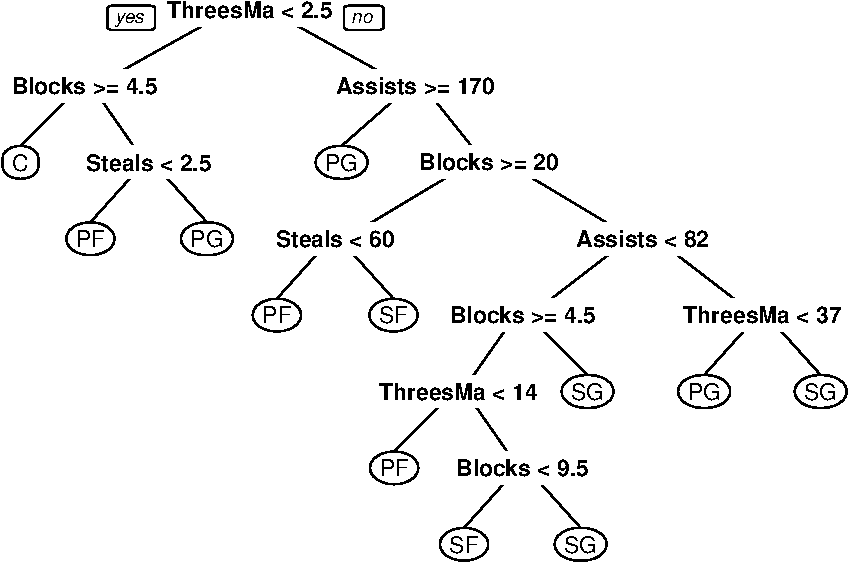
\includegraphics{DataAnalyticsWithR_files/figure-latex/rpart4-1.pdf}

決策樹演算法決定\texttt{節點}的方式如下:

\begin{itemize}
\tightlist
\item
  Gini impurity
\item
  Information gain
\item
  Variance reduction
\end{itemize}

細節可參考\href{https://en.wikipedia.org/wiki/Decision_tree_learning}{維基百科}

\hypertarget{clustering-ux5206ux7fa4}{%
\section{Clustering 分群}\label{clustering-ux5206ux7fa4}}

Clustering 分群的目的是將相近的觀察值作做分群,分群過程中,可能會遇到以下問題:

\begin{itemize}
\tightlist
\item
  如何定義相近?
\item
  如何分群?
\item
  如何視覺化?
\item
  如何解釋分群?
\end{itemize}

\hypertarget{hierarchical-clustering-ux968eux5c64ux5f0fux5206ux7fa4}{%
\subsection{Hierarchical clustering 階層式分群}\label{hierarchical-clustering-ux968eux5c64ux5f0fux5206ux7fa4}}

\begin{itemize}
\tightlist
\item
  An agglomerative approach

  \begin{itemize}
  \tightlist
  \item
    Find closest two things
  \item
    Put them together
  \item
    Find next closest
  \end{itemize}
\item
  Requires

  \begin{itemize}
  \tightlist
  \item
    A defined distance
  \item
    A merging approach
  \end{itemize}
\item
  Produces

  \begin{itemize}
  \tightlist
  \item
    A tree showing how close things are to each other
  \end{itemize}
\end{itemize}

如何定義相近?用距離\texttt{distance}的概念來定義相近。

\begin{itemize}
\tightlist
\item
  Distance or similarity

  \begin{itemize}
  \tightlist
  \item
    Continuous - euclidean distance
  \item
    Continuous - correlation similarity
  \item
    Binary - manhattan distance
  \end{itemize}
\item
  Pick a distance/similarity that makes sense for your problem
\end{itemize}

Example distances - Euclidean

\[\sqrt{(A_1-A_2)^2 + (B_1-B_2)^2 + \ldots + (Z_1-Z_2)^2}\]

Example distances - Manhattan

\[|A_1-A_2| + |B_1-B_2| + \ldots + |Z_1-Z_2|\]

Merging apporach

\begin{itemize}
\item
  Agglomerative 聚合

  \begin{itemize}
  \tightlist
  \item
    Single-linkage:取最小值
  \item
    Complete-linkage:取最大值
  \item
    Average-linkage:取平均值
  \end{itemize}
\end{itemize}

Hierarchical clustering - hp vs.~mpg
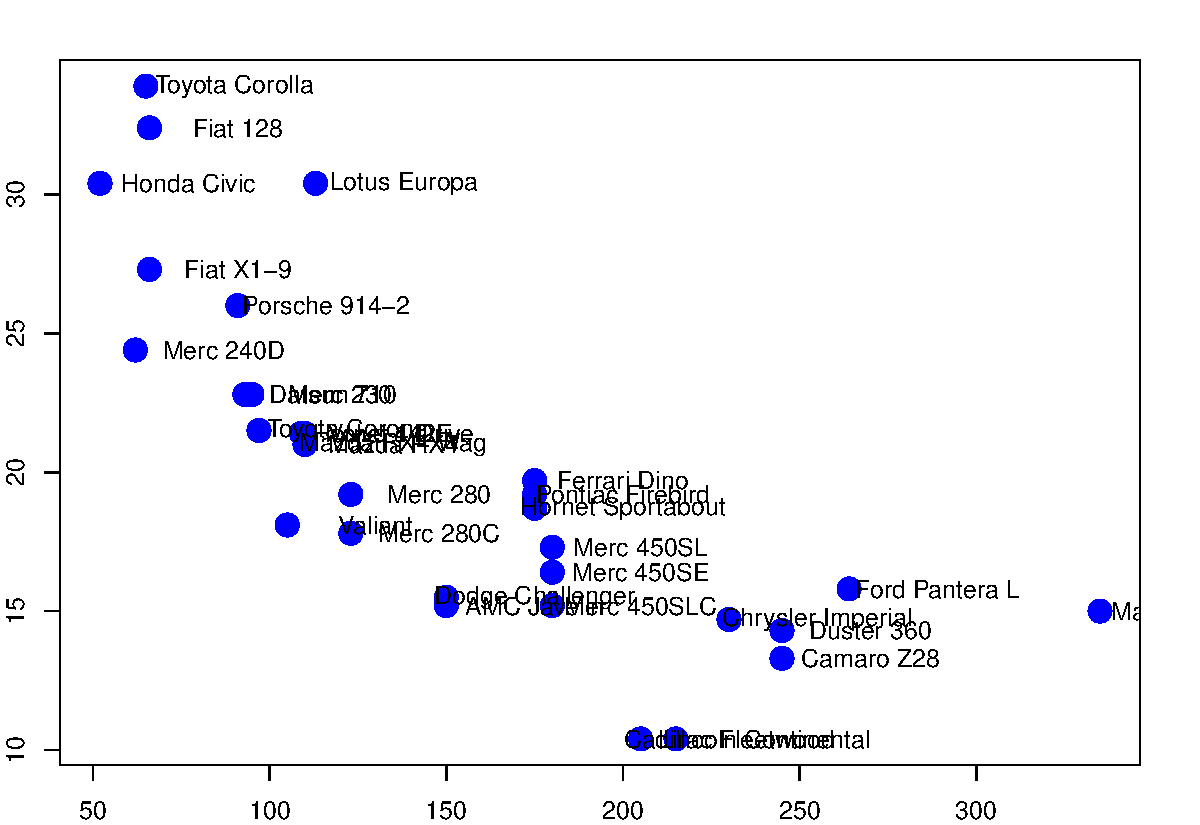
\includegraphics{DataAnalyticsWithR_files/figure-latex/unnamed-chunk-4-1.pdf}

Hierarchical clustering - \#1

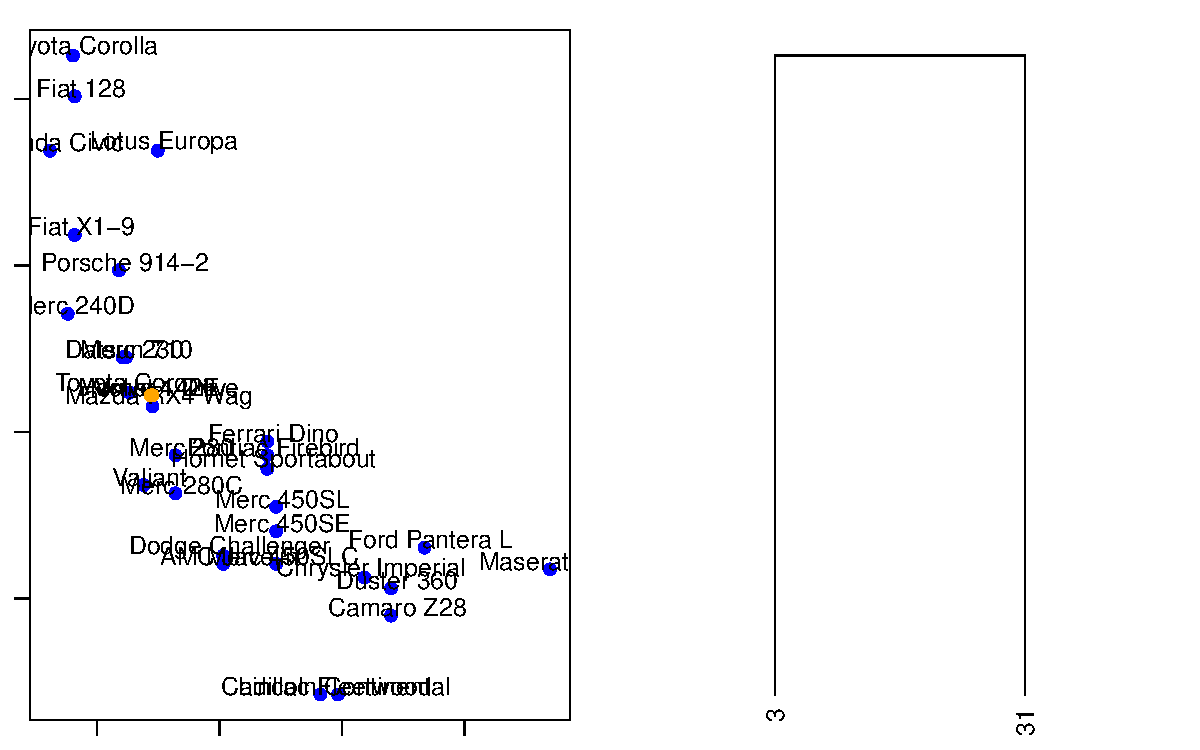
\includegraphics{DataAnalyticsWithR_files/figure-latex/unnamed-chunk-5-1.pdf}

Hierarchical clustering - \#2
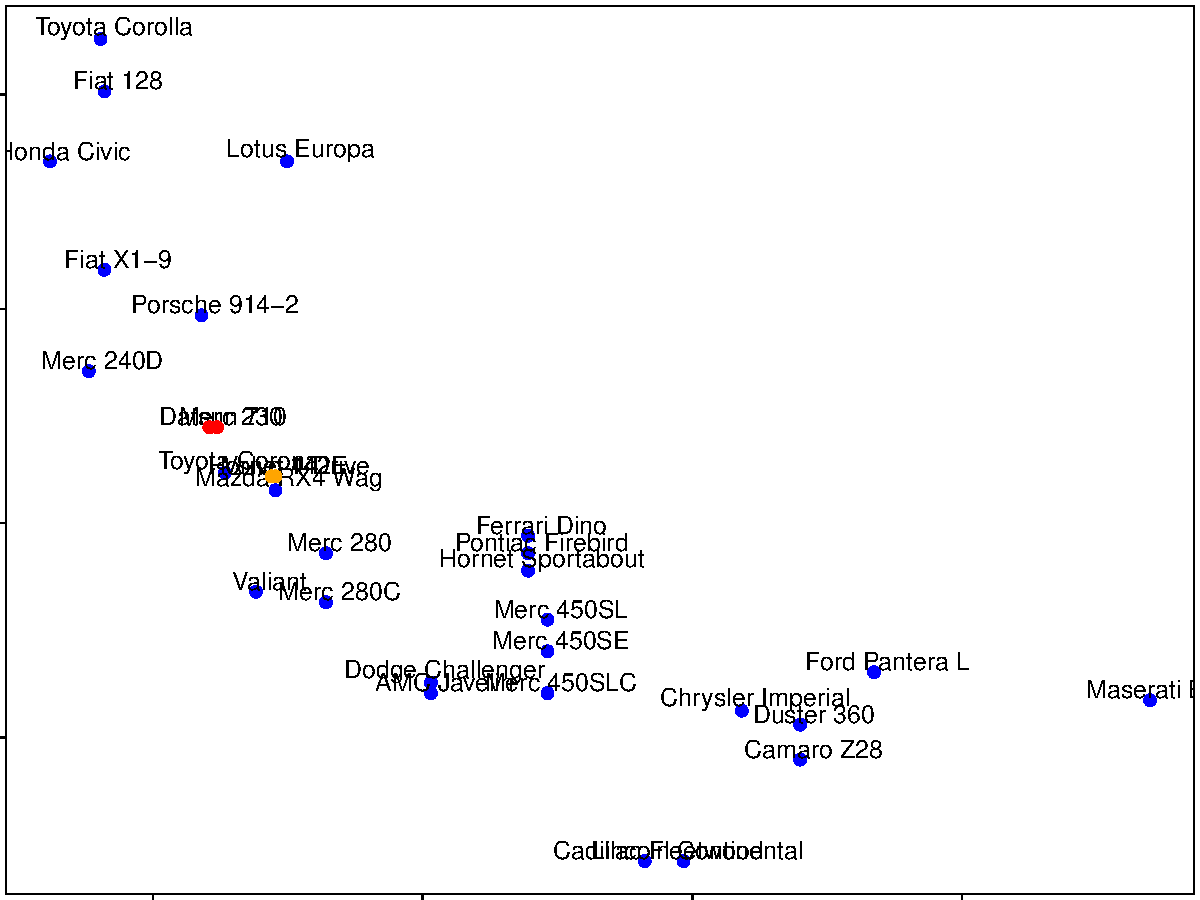
\includegraphics{DataAnalyticsWithR_files/figure-latex/unnamed-chunk-6-1.pdf}

Hierarchical clustering - \#3

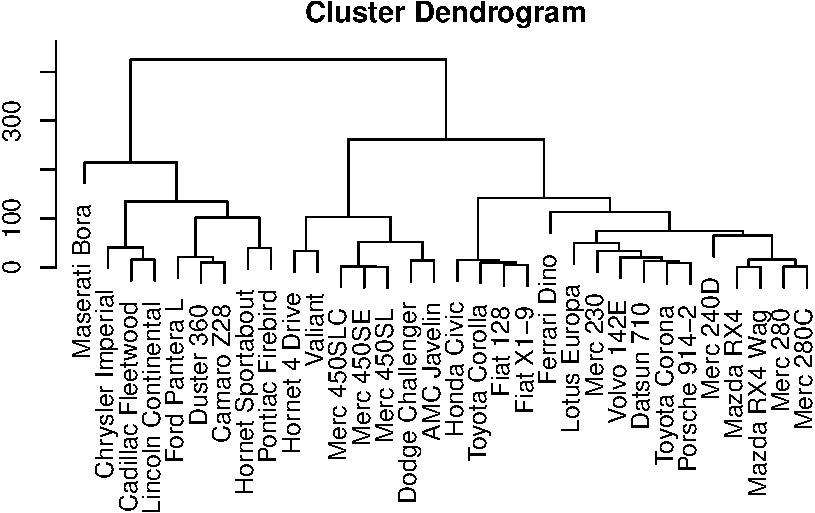
\includegraphics{DataAnalyticsWithR_files/figure-latex/unnamed-chunk-7-1.pdf}

可用\texttt{dist()}函數計算距離,使用method=""設定計算距離的依據

\begin{Shaded}
\begin{Highlighting}[]
\NormalTok{mtcars.mxs<-}\KeywordTok{as.matrix}\NormalTok{(mtcars)}
\NormalTok{d<-}\KeywordTok{dist}\NormalTok{(mtcars.mxs) }\CommentTok{#預設為euclidean}
\KeywordTok{head}\NormalTok{(d)}
\end{Highlighting}
\end{Shaded}

\begin{verbatim}
## [1]   0.6153251  54.9086059  98.1125212 210.3374396  65.4717710 241.4076490
\end{verbatim}

\texttt{dist()}函數可用方法包括:
``euclidean'', ``maximum'', ``manhattan'', ``canberra'', ``binary'' or ``minkowski''

\begin{Shaded}
\begin{Highlighting}[]
\NormalTok{d<-}\KeywordTok{dist}\NormalTok{(mtcars.mxs, }\DataTypeTok{method=}\StringTok{"manhattan"}\NormalTok{) }\CommentTok{#計算manhattan距離}
\KeywordTok{head}\NormalTok{(d)}
\end{Highlighting}
\end{Shaded}

\begin{verbatim}
## [1]   0.815  79.300 108.795 275.430  84.640 347.960
\end{verbatim}

用\texttt{hclust}函數畫圖,必要參數是各觀察值的距離(可用\texttt{dist()}函數計算)

\begin{Shaded}
\begin{Highlighting}[]
\KeywordTok{par}\NormalTok{(}\DataTypeTok{mar=}\KeywordTok{rep}\NormalTok{(}\DecValTok{2}\NormalTok{,}\DecValTok{4}\NormalTok{),}\DataTypeTok{mfrow=}\KeywordTok{c}\NormalTok{(}\DecValTok{1}\NormalTok{,}\DecValTok{1}\NormalTok{))}
\NormalTok{hc<-}\KeywordTok{hclust}\NormalTok{(}\KeywordTok{dist}\NormalTok{(mtcars.mxs)) }\CommentTok{#可用method參數設定聚合方法,預設為complete}
\KeywordTok{plot}\NormalTok{(hc)}
\end{Highlighting}
\end{Shaded}

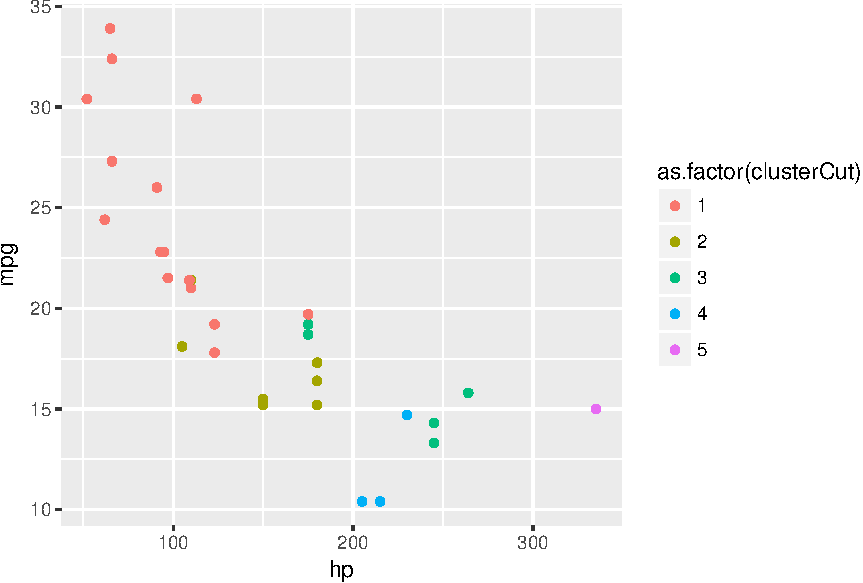
\includegraphics{DataAnalyticsWithR_files/figure-latex/unnamed-chunk-10-1.pdf}

\begin{Shaded}
\begin{Highlighting}[]
\KeywordTok{par}\NormalTok{(}\DataTypeTok{mar=}\KeywordTok{rep}\NormalTok{(}\DecValTok{2}\NormalTok{,}\DecValTok{4}\NormalTok{),}\DataTypeTok{mfrow=}\KeywordTok{c}\NormalTok{(}\DecValTok{1}\NormalTok{,}\DecValTok{1}\NormalTok{))}
\NormalTok{hc<-}\KeywordTok{hclust}\NormalTok{(}\KeywordTok{dist}\NormalTok{(mtcars.mxs),}\DataTypeTok{method=}\StringTok{"average"}\NormalTok{) }\CommentTok{#聚合方法為計算平均距離}
\KeywordTok{plot}\NormalTok{(hc)}
\end{Highlighting}
\end{Shaded}

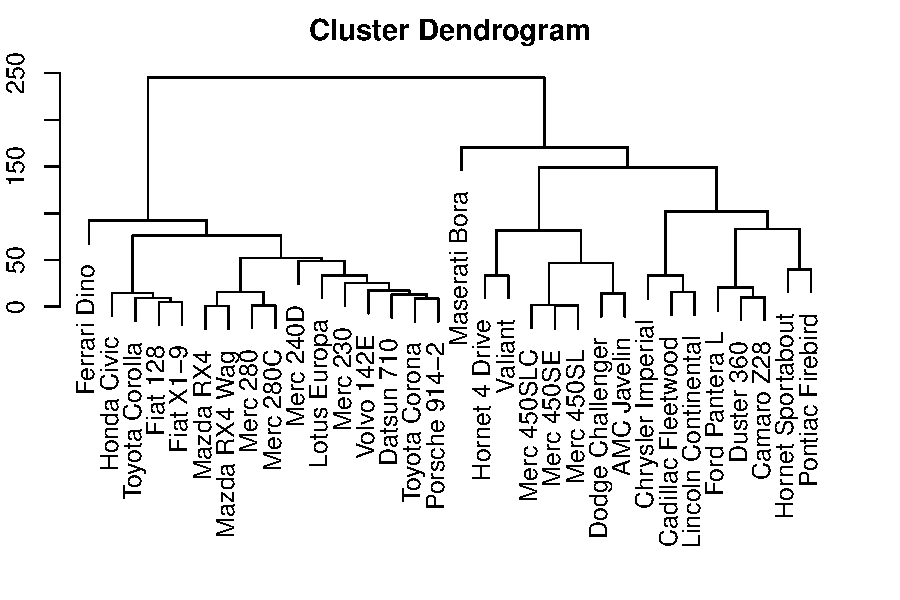
\includegraphics{DataAnalyticsWithR_files/figure-latex/unnamed-chunk-11-1.pdf}

\begin{Shaded}
\begin{Highlighting}[]
\NormalTok{clusterCut <-}\StringTok{ }\KeywordTok{cutree}\NormalTok{(hc, }\DataTypeTok{k=}\DecValTok{5}\NormalTok{) }\CommentTok{#分5群}
\KeywordTok{sort}\NormalTok{(clusterCut)}
\end{Highlighting}
\end{Shaded}

\begin{verbatim}
##           Mazda RX4       Mazda RX4 Wag          Datsun 710 
##                   1                   1                   1 
##           Merc 240D            Merc 230            Merc 280 
##                   1                   1                   1 
##           Merc 280C            Fiat 128         Honda Civic 
##                   1                   1                   1 
##      Toyota Corolla       Toyota Corona           Fiat X1-9 
##                   1                   1                   1 
##       Porsche 914-2        Lotus Europa        Ferrari Dino 
##                   1                   1                   1 
##          Volvo 142E      Hornet 4 Drive             Valiant 
##                   1                   2                   2 
##          Merc 450SE          Merc 450SL         Merc 450SLC 
##                   2                   2                   2 
##    Dodge Challenger         AMC Javelin   Hornet Sportabout 
##                   2                   2                   3 
##          Duster 360          Camaro Z28    Pontiac Firebird 
##                   3                   3                   3 
##      Ford Pantera L  Cadillac Fleetwood Lincoln Continental 
##                   3                   4                   4 
##   Chrysler Imperial       Maserati Bora 
##                   4                   5
\end{verbatim}

\begin{Shaded}
\begin{Highlighting}[]
\KeywordTok{ggplot}\NormalTok{()}\OperatorTok{+}\KeywordTok{geom_point}\NormalTok{(}\DataTypeTok{data=}\NormalTok{mtcars,}
                    \KeywordTok{aes}\NormalTok{(}\DataTypeTok{x=}\NormalTok{hp,}\DataTypeTok{y=}\NormalTok{mpg,}\DataTypeTok{color=}\KeywordTok{as.factor}\NormalTok{(clusterCut)))}
\end{Highlighting}
\end{Shaded}

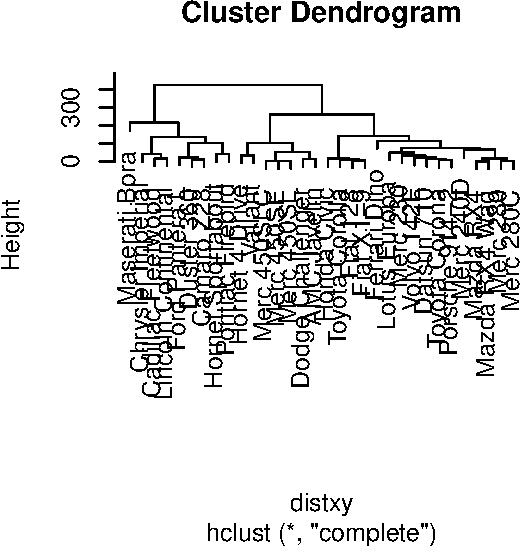
\includegraphics{DataAnalyticsWithR_files/figure-latex/unnamed-chunk-13-1.pdf}

\begin{Shaded}
\begin{Highlighting}[]
\NormalTok{clusterCut <-}\StringTok{ }\KeywordTok{cutree}\NormalTok{(hc,}\DataTypeTok{h =}\DecValTok{4}\NormalTok{) }\CommentTok{#切在高度=4的地方(距離=4)}
\KeywordTok{sort}\NormalTok{(clusterCut)}
\end{Highlighting}
\end{Shaded}

\begin{verbatim}
##           Mazda RX4       Mazda RX4 Wag          Datsun 710 
##                   1                   1                   2 
##      Hornet 4 Drive   Hornet Sportabout             Valiant 
##                   3                   4                   5 
##          Duster 360           Merc 240D            Merc 230 
##                   6                   7                   8 
##            Merc 280           Merc 280C          Merc 450SE 
##                   9                   9                  10 
##          Merc 450SL         Merc 450SLC  Cadillac Fleetwood 
##                  10                  10                  11 
## Lincoln Continental   Chrysler Imperial            Fiat 128 
##                  12                  13                  14 
##         Honda Civic      Toyota Corolla       Toyota Corona 
##                  15                  16                  17 
##    Dodge Challenger         AMC Javelin          Camaro Z28 
##                  18                  19                  20 
##    Pontiac Firebird           Fiat X1-9       Porsche 914-2 
##                  21                  22                  23 
##        Lotus Europa      Ford Pantera L        Ferrari Dino 
##                  24                  25                  26 
##       Maserati Bora          Volvo 142E 
##                  27                  28
\end{verbatim}

\begin{Shaded}
\begin{Highlighting}[]
\KeywordTok{par}\NormalTok{(}\DataTypeTok{mar=}\KeywordTok{rep}\NormalTok{(}\FloatTok{0.2}\NormalTok{,}\DecValTok{4}\NormalTok{),}\DataTypeTok{mfrow=}\KeywordTok{c}\NormalTok{(}\DecValTok{1}\NormalTok{,}\DecValTok{1}\NormalTok{))}
\KeywordTok{heatmap}\NormalTok{(mtcars.mxs)}
\end{Highlighting}
\end{Shaded}

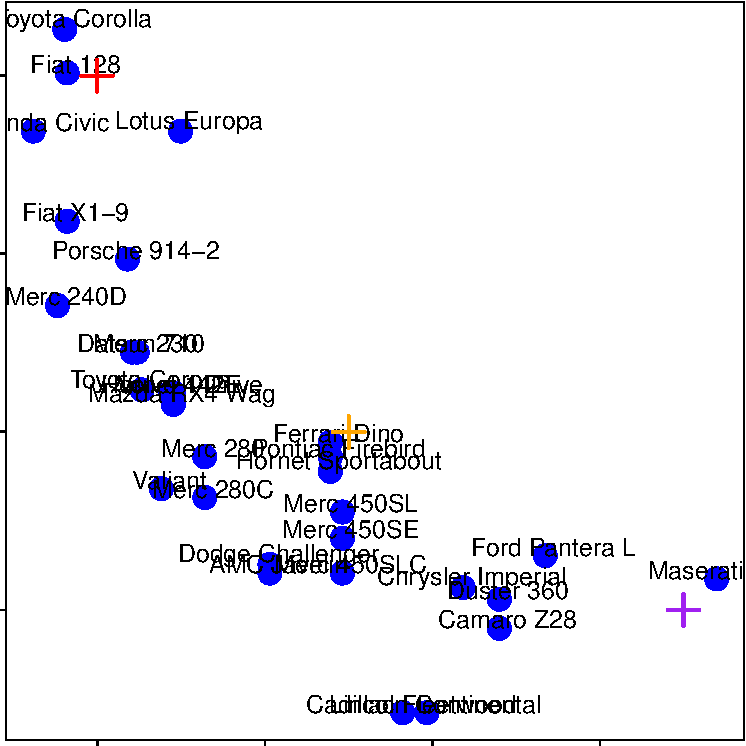
\includegraphics{DataAnalyticsWithR_files/figure-latex/unnamed-chunk-15-1.pdf}

\begin{Shaded}
\begin{Highlighting}[]
\NormalTok{distxy <-}\StringTok{ }\KeywordTok{dist}\NormalTok{(mtcars.mxs)}
\NormalTok{hClustering <-}\StringTok{ }\KeywordTok{hclust}\NormalTok{(distxy)}
\KeywordTok{plot}\NormalTok{(hClustering)}
\end{Highlighting}
\end{Shaded}

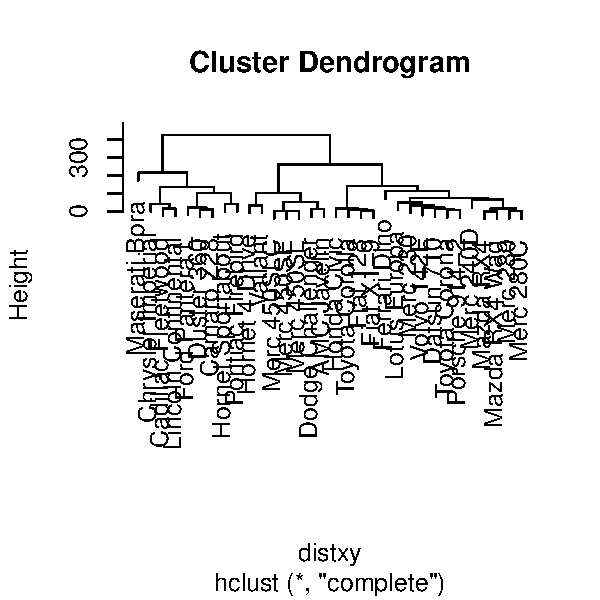
\includegraphics{DataAnalyticsWithR_files/figure-latex/unnamed-chunk-16-1.pdf}

Hierarchical clustering: summary
- 可快速瀏覽觀察值與各欄位的關係

\begin{itemize}
\tightlist
\item
  分群結果可能被以下參數影響:

  \begin{itemize}
  \tightlist
  \item
    計算距離的方法
  \item
    分群依據
  \item
    更改數值的大小
  \end{itemize}
\item
  可能會遇到的問題:

  \begin{itemize}
  \tightlist
  \item
    有時會不太清楚要如何切割分群結果
  \end{itemize}
\end{itemize}

\hypertarget{k-means-clustering}{%
\subsection{K-means clustering}\label{k-means-clustering}}

\begin{itemize}
\tightlist
\item
  執行步驟

  \begin{itemize}
  \tightlist
  \item
    指定要分幾群
  \item
    計算每一群的中心點
  \item
    將各個物件/觀察值指定給最近的中心點
  \item
    依照新的分群計算新的中心點
  \end{itemize}
\item
  輸入

  \begin{itemize}
  \tightlist
  \item
    計算距離的資料(數值)
  \item
    要分成幾群 \# of clusters
  \item
    預設個群的中間點位置
  \end{itemize}
\item
  產出

  \begin{itemize}
  \tightlist
  \item
    計算出每'群`的中心點
  \item
    指定每個觀察值所在的'群`
  \end{itemize}
\end{itemize}

\begin{Shaded}
\begin{Highlighting}[]
\NormalTok{x<-}\KeywordTok{scale}\NormalTok{(mtcars}\OperatorTok{$}\NormalTok{hp[}\OperatorTok{-}\DecValTok{1}\NormalTok{]);y<-}\KeywordTok{scale}\NormalTok{(mtcars}\OperatorTok{$}\NormalTok{mpg[}\OperatorTok{-}\DecValTok{1}\NormalTok{])}
\KeywordTok{plot}\NormalTok{(x,y,}\DataTypeTok{col=}\StringTok{"blue"}\NormalTok{,}\DataTypeTok{pch=}\DecValTok{19}\NormalTok{,}\DataTypeTok{cex=}\DecValTok{2}\NormalTok{)}
\KeywordTok{text}\NormalTok{(x}\FloatTok{+0.05}\NormalTok{,y}\FloatTok{+0.05}\NormalTok{,}\DataTypeTok{labels=}\NormalTok{labelCar)}
\end{Highlighting}
\end{Shaded}

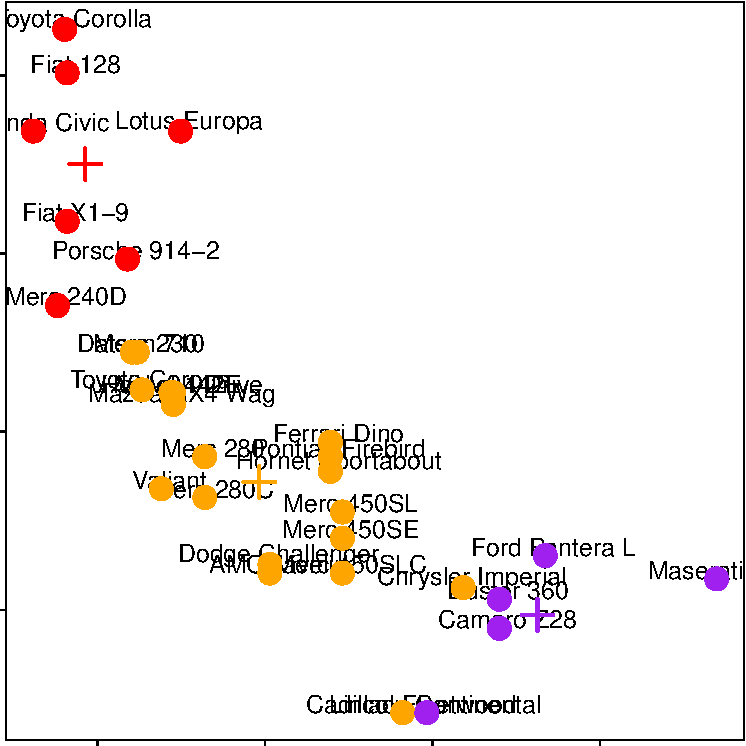
\includegraphics{DataAnalyticsWithR_files/figure-latex/unnamed-chunk-17-1.pdf}

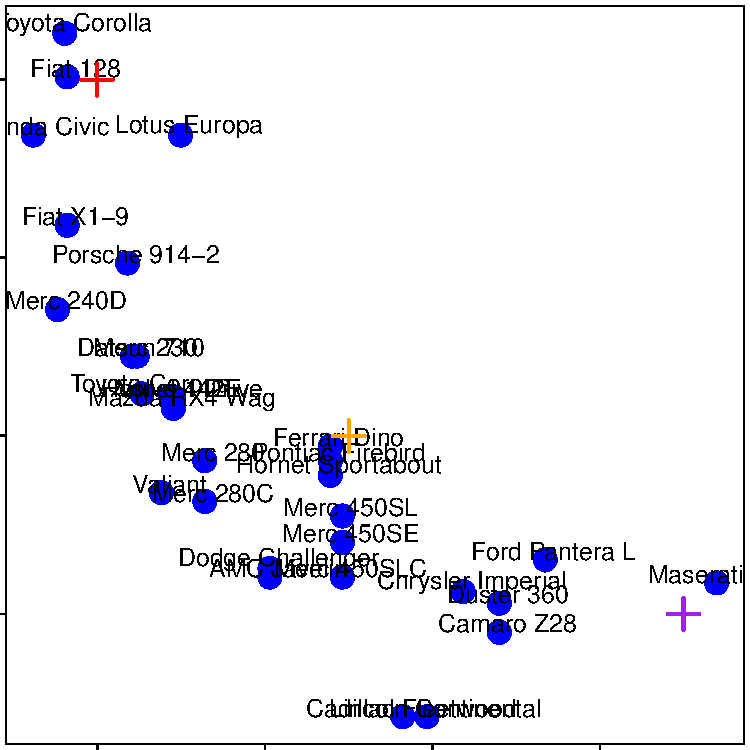
\includegraphics{DataAnalyticsWithR_files/figure-latex/unnamed-chunk-18-1.pdf}

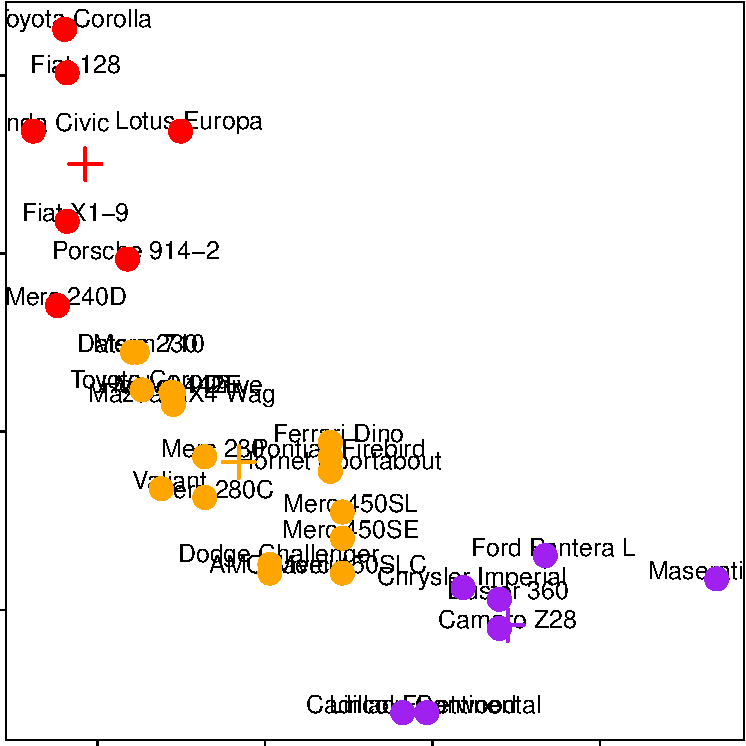
\includegraphics{DataAnalyticsWithR_files/figure-latex/unnamed-chunk-19-1.pdf}

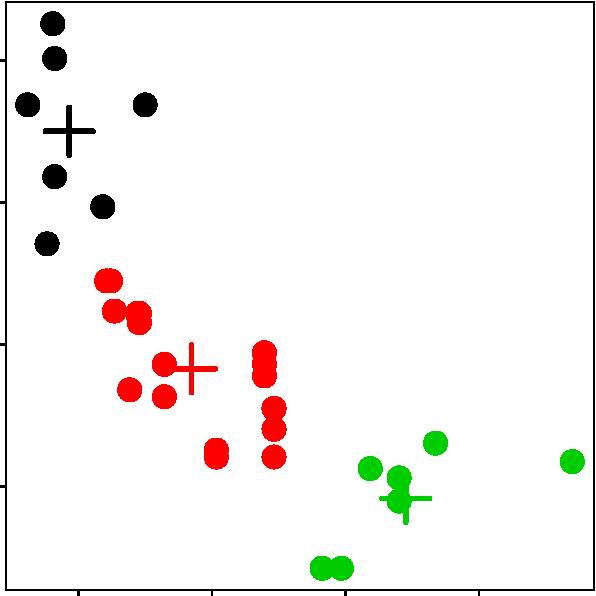
\includegraphics{DataAnalyticsWithR_files/figure-latex/unnamed-chunk-20-1.pdf}

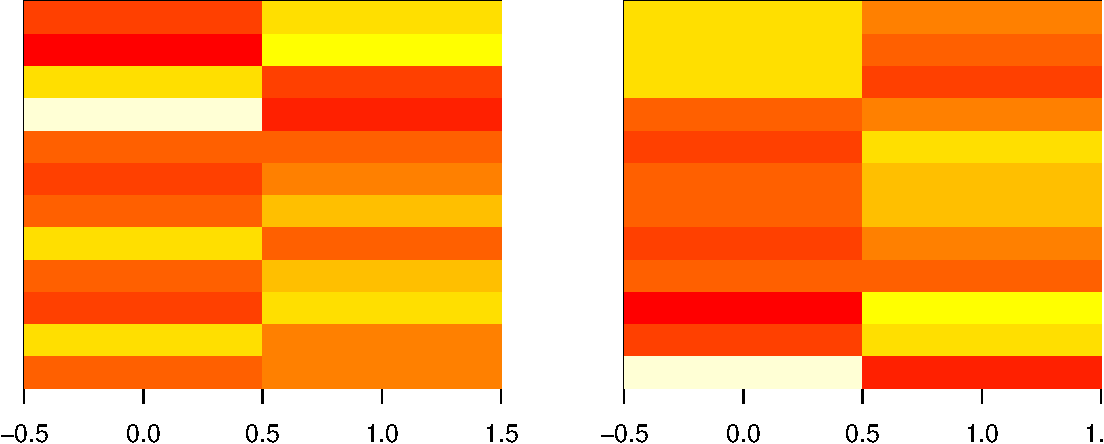
\includegraphics{DataAnalyticsWithR_files/figure-latex/unnamed-chunk-21-1.pdf}

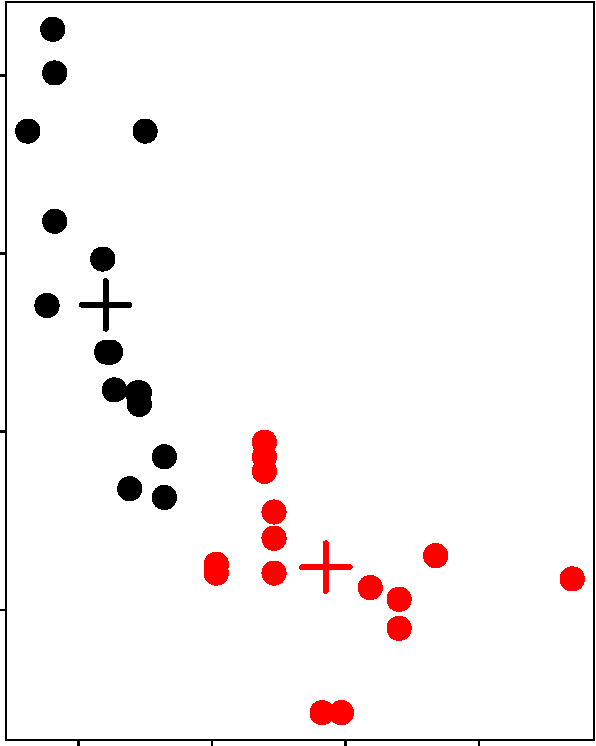
\includegraphics{DataAnalyticsWithR_files/figure-latex/unnamed-chunk-22-1.pdf}

\texttt{kmeans()}

\begin{itemize}
\tightlist
\item
  Important parameters: \texttt{x}, \texttt{centers}, \texttt{iter.max}, \texttt{nstart}
\end{itemize}

\begin{Shaded}
\begin{Highlighting}[]
\NormalTok{dataFrame <-}\StringTok{ }\KeywordTok{data.frame}\NormalTok{(x,y)}
\NormalTok{kmeansObj <-}\StringTok{ }\KeywordTok{kmeans}\NormalTok{(dataFrame,}\DataTypeTok{centers=}\DecValTok{3}\NormalTok{)}
\KeywordTok{names}\NormalTok{(kmeansObj)}
\end{Highlighting}
\end{Shaded}

\begin{verbatim}
## [1] "cluster"      "centers"      "totss"        "withinss"    
## [5] "tot.withinss" "betweenss"    "size"         "iter"        
## [9] "ifault"
\end{verbatim}

\begin{Shaded}
\begin{Highlighting}[]
\NormalTok{kmeansObj}\OperatorTok{$}\NormalTok{cluster}
\end{Highlighting}
\end{Shaded}

\begin{verbatim}
##  [1] 2 1 2 2 2 3 1 1 2 2 2 2 2 3 3 3 1 1 1 2 2 2 3 2 1 1 1 3 2 3 2
\end{verbatim}

\begin{Shaded}
\begin{Highlighting}[]
\KeywordTok{par}\NormalTok{(}\DataTypeTok{mar=}\KeywordTok{rep}\NormalTok{(}\FloatTok{0.2}\NormalTok{,}\DecValTok{4}\NormalTok{))}
\KeywordTok{plot}\NormalTok{(x,y,}\DataTypeTok{col=}\NormalTok{kmeansObj}\OperatorTok{$}\NormalTok{cluster,}\DataTypeTok{pch=}\DecValTok{19}\NormalTok{,}\DataTypeTok{cex=}\DecValTok{2}\NormalTok{)}
\KeywordTok{points}\NormalTok{(kmeansObj}\OperatorTok{$}\NormalTok{centers,}\DataTypeTok{col=}\DecValTok{1}\OperatorTok{:}\DecValTok{3}\NormalTok{,}\DataTypeTok{pch=}\DecValTok{3}\NormalTok{,}\DataTypeTok{cex=}\DecValTok{3}\NormalTok{,}\DataTypeTok{lwd=}\DecValTok{3}\NormalTok{)}
\end{Highlighting}
\end{Shaded}

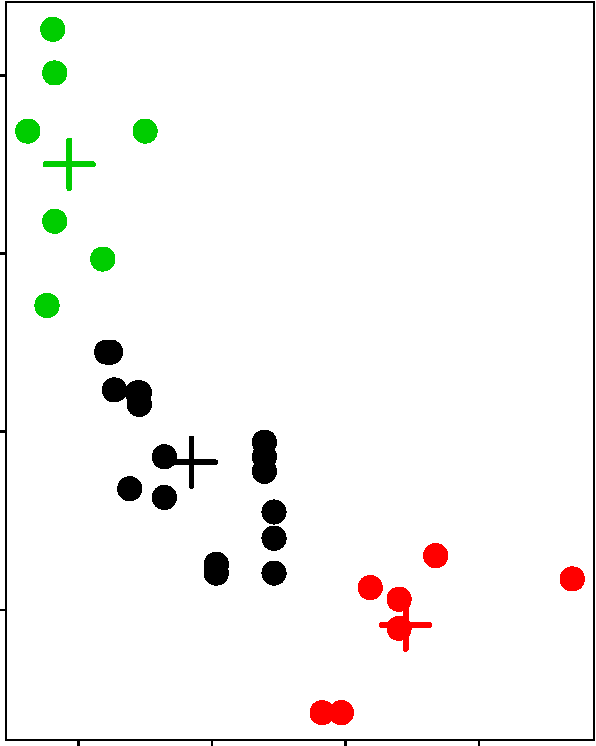
\includegraphics{DataAnalyticsWithR_files/figure-latex/unnamed-chunk-23-1.pdf}

Heatmaps

\begin{Shaded}
\begin{Highlighting}[]
\KeywordTok{set.seed}\NormalTok{(}\DecValTok{1234}\NormalTok{)}
\NormalTok{dataMatrix <-}\StringTok{ }\KeywordTok{as.matrix}\NormalTok{(dataFrame)[}\KeywordTok{sample}\NormalTok{(}\DecValTok{1}\OperatorTok{:}\DecValTok{12}\NormalTok{),]}
\NormalTok{kmeansObj <-}\StringTok{ }\KeywordTok{kmeans}\NormalTok{(dataMatrix,}\DataTypeTok{centers=}\DecValTok{3}\NormalTok{)}
\KeywordTok{par}\NormalTok{(}\DataTypeTok{mfrow=}\KeywordTok{c}\NormalTok{(}\DecValTok{1}\NormalTok{,}\DecValTok{2}\NormalTok{), }\DataTypeTok{mar =} \KeywordTok{c}\NormalTok{(}\DecValTok{2}\NormalTok{, }\DecValTok{4}\NormalTok{, }\FloatTok{0.1}\NormalTok{, }\FloatTok{0.1}\NormalTok{))}
\KeywordTok{image}\NormalTok{(}\KeywordTok{t}\NormalTok{(dataMatrix)[,}\KeywordTok{nrow}\NormalTok{(dataMatrix)}\OperatorTok{:}\DecValTok{1}\NormalTok{],}\DataTypeTok{yaxt=}\StringTok{"n"}\NormalTok{)}
\KeywordTok{image}\NormalTok{(}\KeywordTok{t}\NormalTok{(dataMatrix)[,}\KeywordTok{order}\NormalTok{(kmeansObj}\OperatorTok{$}\NormalTok{cluster)],}\DataTypeTok{yaxt=}\StringTok{"n"}\NormalTok{)}
\end{Highlighting}
\end{Shaded}

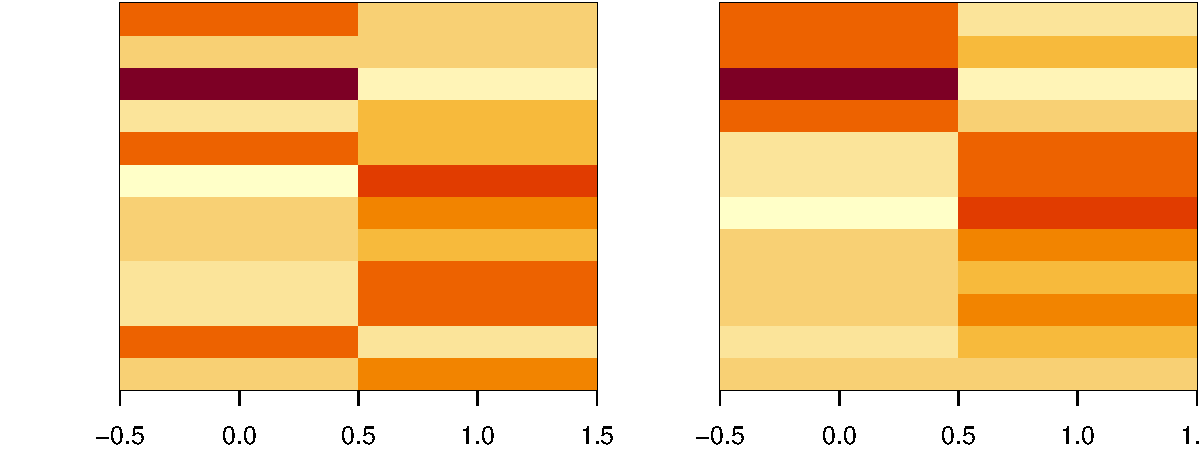
\includegraphics{DataAnalyticsWithR_files/figure-latex/unnamed-chunk-24-1.pdf}

K-means注意事項

\begin{itemize}
\tightlist
\item
  需要決定\# of clusters

  \begin{itemize}
  \tightlist
  \item
    用眼睛/人工/特殊要求選
  \item
    用 cross validation/information theory選
  \item
    \href{http://en.wikipedia.org/wiki/Determining_the_number_of_clusters_in_a_data_set}{Determining the number of clusters}
  \end{itemize}
\item
  K-means 沒有一定的結果

  \begin{itemize}
  \tightlist
  \item
    不同的 \# of clusters
  \item
    不同的 \# of iterations
  \end{itemize}
\end{itemize}

\texttt{kmeans()}, k=2

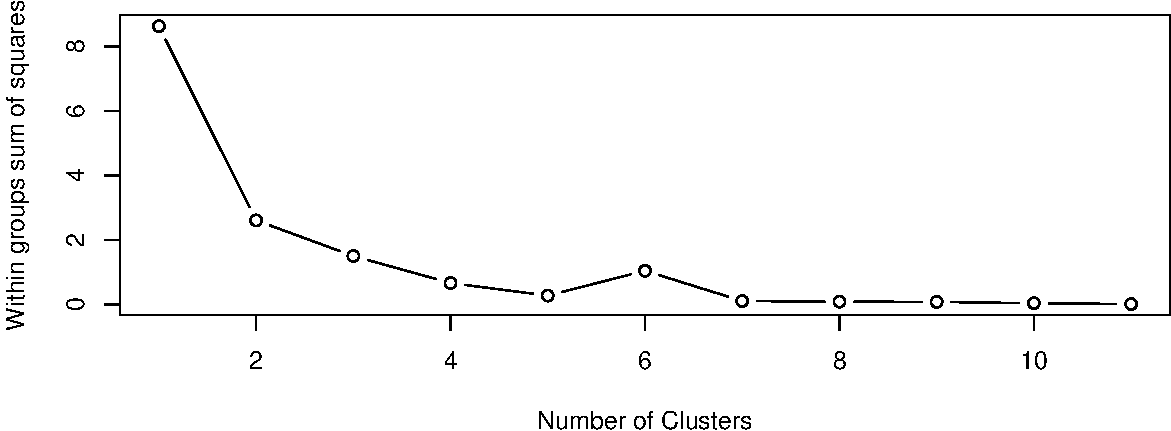
\includegraphics{DataAnalyticsWithR_files/figure-latex/unnamed-chunk-25-1.pdf}

\texttt{kmeans()}, k=3

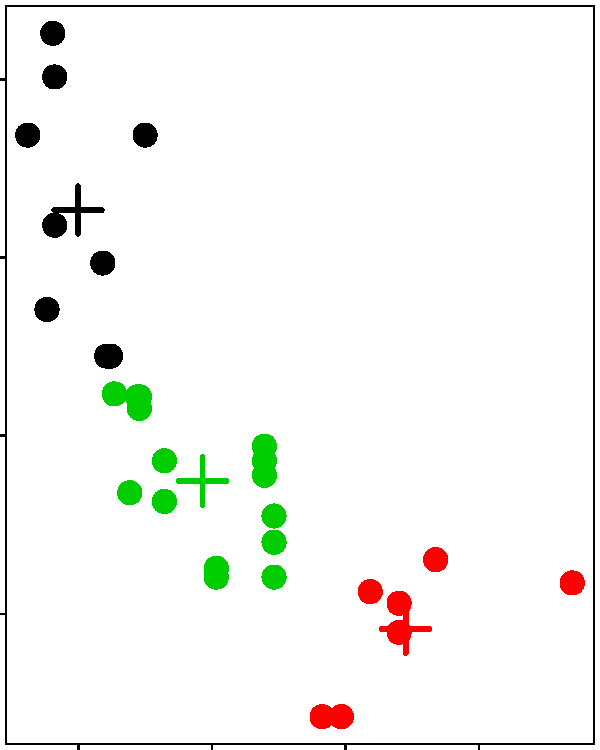
\includegraphics{DataAnalyticsWithR_files/figure-latex/unnamed-chunk-26-1.pdf}

\texttt{kmeans()}, k=4

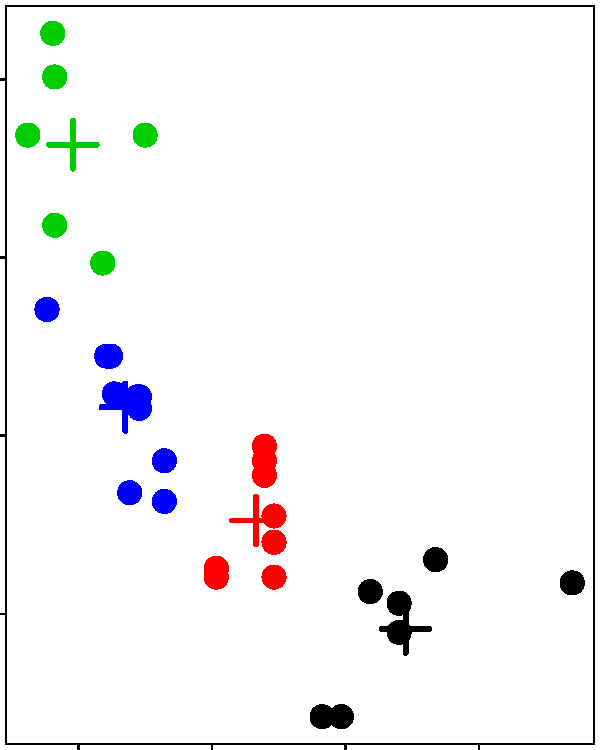
\includegraphics{DataAnalyticsWithR_files/figure-latex/unnamed-chunk-27-1.pdf}

\hypertarget{association-rules-ux95dcux806fux5f0fux898fux5247}{%
\section{Association Rules 關聯式規則}\label{association-rules-ux95dcux806fux5f0fux898fux5247}}

\textbf{關聯式規則}用於從大量數據中挖掘出有價值的數據項之間的相關關係,原則為不考慮項目的次序,而僅考慮其組合。著名的\texttt{購物籃分析\ (Market\ Basket\ Analysis)}即為關聯式規則分析的應用。而\textbf{Apriori演算法}是挖掘\texttt{布林關聯規則} (Boolean association rules) 頻繁項集的算法,在R中,可以使用\texttt{arules}\citep{R-arules} 套件來執行關聯式規則分析。

以下以超市資料為例,使用關聯式規則分析執行購物籃分析。

首先先讀入超市消費資料

\begin{Shaded}
\begin{Highlighting}[]
\CommentTok{# Load the libraries}
\ControlFlowTok{if}\NormalTok{ (}\OperatorTok{!}\KeywordTok{require}\NormalTok{(}\StringTok{'arules'}\NormalTok{))\{}
  \KeywordTok{install.packages}\NormalTok{(}\StringTok{"arules"}\NormalTok{);}
  \KeywordTok{library}\NormalTok{(arules) }\CommentTok{#for Apriori演算法}
\NormalTok{\}}
\ControlFlowTok{if}\NormalTok{ (}\OperatorTok{!}\KeywordTok{require}\NormalTok{(}\StringTok{'datasets'}\NormalTok{))\{}
  \KeywordTok{install.packages}\NormalTok{(}\StringTok{"datasets"}\NormalTok{);}
  \KeywordTok{library}\NormalTok{(datasets) }\CommentTok{#for Groceries data}
\NormalTok{\}}
\KeywordTok{data}\NormalTok{(Groceries) }\CommentTok{# Load the data set}
\NormalTok{Groceries}\OperatorTok{@}\NormalTok{data}\OperatorTok{@}\NormalTok{Dim }\CommentTok{#169 種商品,9835筆交易資料}
\end{Highlighting}
\end{Shaded}

\begin{verbatim}
## [1]  169 9835
\end{verbatim}

超市資料的原始樣貌為:

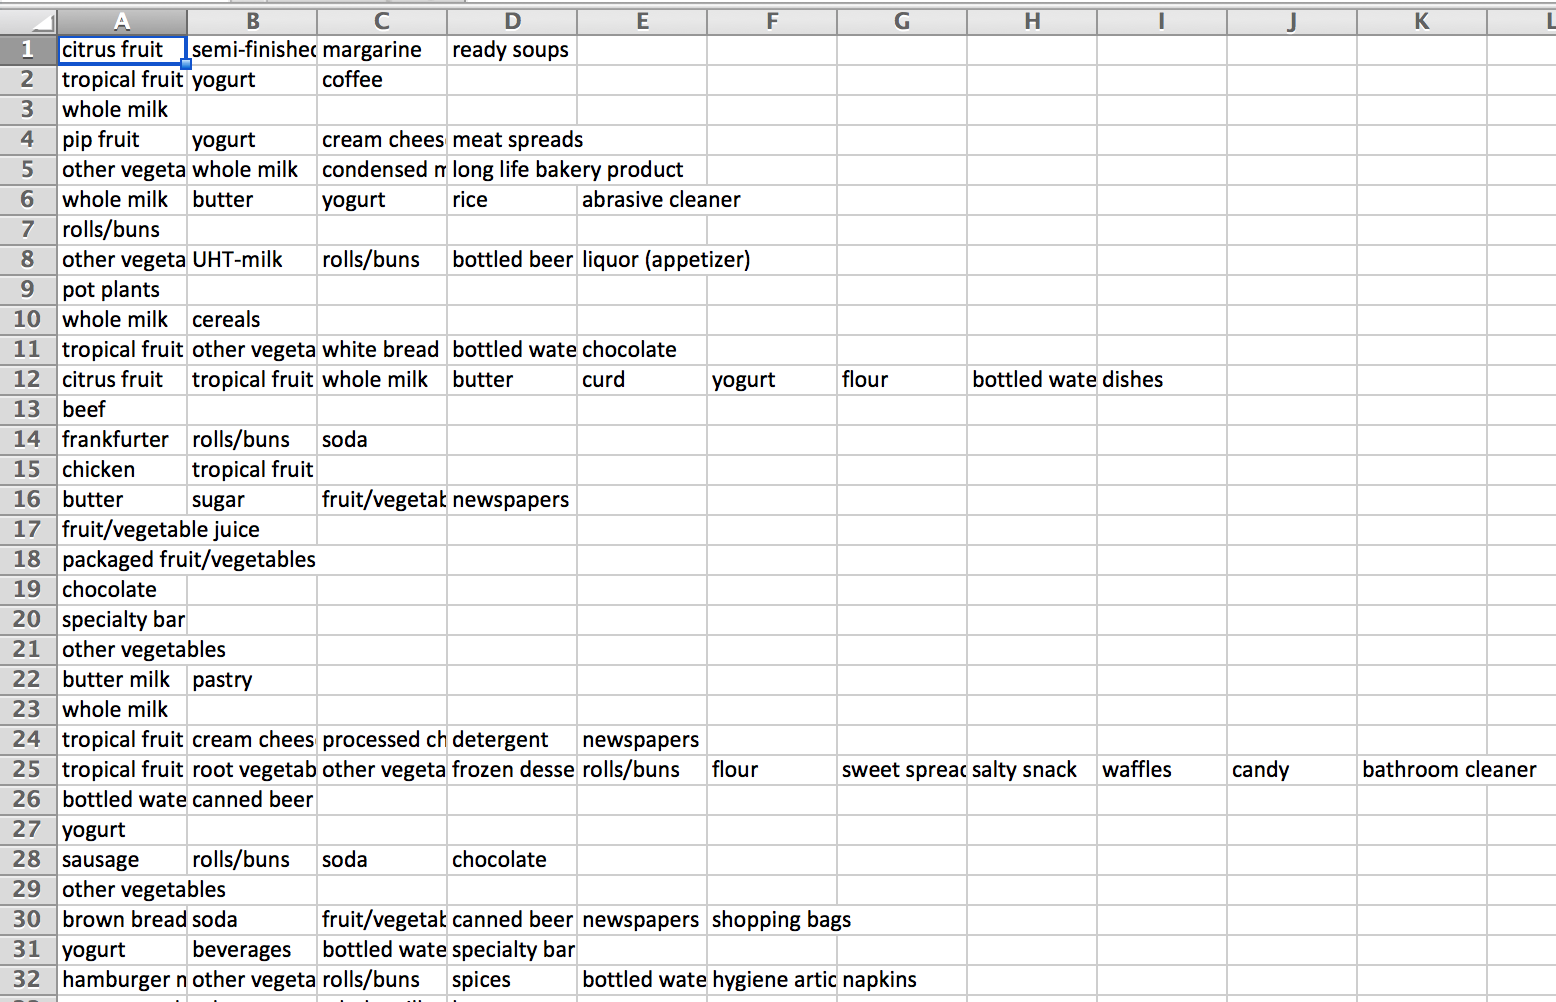
\includegraphics[width=21.61in]{figure/groceries}

可使用arules套件中的apriori函數來實作apriori演算法

\begin{Shaded}
\begin{Highlighting}[]
\CommentTok{# Get the rules}
\NormalTok{rules <-}\StringTok{ }\KeywordTok{apriori}\NormalTok{(Groceries, }\CommentTok{# data= Groceries}
                 \DataTypeTok{parameter =} \KeywordTok{list}\NormalTok{(}\DataTypeTok{supp =} \FloatTok{0.001}\NormalTok{, }\DataTypeTok{conf =} \FloatTok{0.8}\NormalTok{), }\CommentTok{#參數最低限度}
                 \DataTypeTok{control =} \KeywordTok{list}\NormalTok{(}\DataTypeTok{verbose=}\NormalTok{F)) }\CommentTok{#不要顯示output}
\KeywordTok{options}\NormalTok{(}\DataTypeTok{digits=}\DecValTok{2}\NormalTok{) }\CommentTok{# Only 2 digits}
\KeywordTok{inspect}\NormalTok{(rules[}\DecValTok{1}\OperatorTok{:}\DecValTok{5}\NormalTok{]) }\CommentTok{# Show the top 5 rules}
\end{Highlighting}
\end{Shaded}

\begin{verbatim}
##     lhs                        rhs            support confidence lift
## [1] {liquor,red/blush wine} => {bottled beer} 0.0019  0.90       11.2
## [2] {curd,cereals}          => {whole milk}   0.0010  0.91        3.6
## [3] {yogurt,cereals}        => {whole milk}   0.0017  0.81        3.2
## [4] {butter,jam}            => {whole milk}   0.0010  0.83        3.3
## [5] {soups,bottled beer}    => {whole milk}   0.0011  0.92        3.6
##     count
## [1] 19   
## [2] 10   
## [3] 17   
## [4] 10   
## [5] 11
\end{verbatim}

根據計算結果,解讀模型的方法如下:

啤酒=\textgreater 尿布

\begin{itemize}
\tightlist
\item
  \texttt{Support}: 一次交易中,包括規則內的物品的機率。買啤酒同時買尿布的機率。交集
\item
  \texttt{Confidence}: 包含左邊物品A的交易也會包含右邊物品B的條件機率。在買了啤酒的顧客中,有買尿布的比例。
\item
  \texttt{Lift}: 規則的信心比期望值高多少。(買了啤酒以後,有買尿布的機率)/(在所有顧客群中買尿布的機率)

  \begin{itemize}
  \tightlist
  \item
    \texttt{lift}=1: items on the left and right are independent.
  \end{itemize}
\end{itemize}

可用排序功能排序後,列出最有關連(confidence最高)的幾條規則

\begin{Shaded}
\begin{Highlighting}[]
\NormalTok{rules<-}\KeywordTok{sort}\NormalTok{(rules, }\DataTypeTok{by=}\StringTok{"confidence"}\NormalTok{, }\DataTypeTok{decreasing=}\OtherTok{TRUE}\NormalTok{) }\CommentTok{#按照confidence排序}
\KeywordTok{inspect}\NormalTok{(rules[}\DecValTok{1}\OperatorTok{:}\DecValTok{5}\NormalTok{]) }\CommentTok{# Show the top 5 rules}
\end{Highlighting}
\end{Shaded}

\begin{verbatim}
##     lhs                     rhs          support confidence lift count
## [1] {rice,                                                            
##      sugar}              => {whole milk}  0.0012          1  3.9    12
## [2] {canned fish,                                                     
##      hygiene articles}   => {whole milk}  0.0011          1  3.9    11
## [3] {root vegetables,                                                 
##      butter,                                                          
##      rice}               => {whole milk}  0.0010          1  3.9    10
## [4] {root vegetables,                                                 
##      whipped/sour cream,                                              
##      flour}              => {whole milk}  0.0017          1  3.9    17
## [5] {butter,                                                          
##      soft cheese,                                                     
##      domestic eggs}      => {whole milk}  0.0010          1  3.9    10
\end{verbatim}

特別針對某項商品(右側變數),像是:買了什麼東西的人,會買\texttt{牛奶}呢?

\begin{Shaded}
\begin{Highlighting}[]
\NormalTok{rulesR<-}\KeywordTok{apriori}\NormalTok{(}\DataTypeTok{data=}\NormalTok{Groceries, }\DataTypeTok{parameter=}\KeywordTok{list}\NormalTok{(}\DataTypeTok{supp=}\FloatTok{0.001}\NormalTok{,}\DataTypeTok{conf =} \FloatTok{0.08}\NormalTok{),}
        \DataTypeTok{appearance =} \KeywordTok{list}\NormalTok{(}\DataTypeTok{default=}\StringTok{"lhs"}\NormalTok{,}\DataTypeTok{rhs=}\StringTok{"whole milk"}\NormalTok{), }\CommentTok{#設定右邊一定要是牛奶}
        \DataTypeTok{control =} \KeywordTok{list}\NormalTok{(}\DataTypeTok{verbose=}\NormalTok{F)) }\CommentTok{#不要顯示output}
\NormalTok{rulesR<-}\KeywordTok{sort}\NormalTok{(rulesR, }\DataTypeTok{decreasing=}\OtherTok{TRUE}\NormalTok{,}\DataTypeTok{by=}\StringTok{"confidence"}\NormalTok{) }\CommentTok{#按照confidence排序}
\KeywordTok{inspect}\NormalTok{(rulesR[}\DecValTok{1}\OperatorTok{:}\DecValTok{5}\NormalTok{]) }\CommentTok{# Show the top 5 rules}
\end{Highlighting}
\end{Shaded}

\begin{verbatim}
##     lhs                     rhs          support confidence lift count
## [1] {rice,                                                            
##      sugar}              => {whole milk}  0.0012          1  3.9    12
## [2] {canned fish,                                                     
##      hygiene articles}   => {whole milk}  0.0011          1  3.9    11
## [3] {root vegetables,                                                 
##      butter,                                                          
##      rice}               => {whole milk}  0.0010          1  3.9    10
## [4] {root vegetables,                                                 
##      whipped/sour cream,                                              
##      flour}              => {whole milk}  0.0017          1  3.9    17
## [5] {butter,                                                          
##      soft cheese,                                                     
##      domestic eggs}      => {whole milk}  0.0010          1  3.9    10
\end{verbatim}

特別針對某項商品(左側變數),像是:買了\texttt{牛奶}的人,會買什麼呢?

\begin{Shaded}
\begin{Highlighting}[]
\NormalTok{rulesL<-}\KeywordTok{apriori}\NormalTok{(}\DataTypeTok{data=}\NormalTok{Groceries, }\DataTypeTok{parameter=}\KeywordTok{list}\NormalTok{(}\DataTypeTok{supp=}\FloatTok{0.001}\NormalTok{,}\DataTypeTok{conf =} \FloatTok{0.15}\NormalTok{,}\DataTypeTok{minlen=}\DecValTok{2}\NormalTok{),}
        \DataTypeTok{appearance =} \KeywordTok{list}\NormalTok{(}\DataTypeTok{default=}\StringTok{"rhs"}\NormalTok{,}\DataTypeTok{lhs=}\StringTok{"whole milk"}\NormalTok{), }\CommentTok{#設定左邊一定要是牛奶}
        \DataTypeTok{control =} \KeywordTok{list}\NormalTok{(}\DataTypeTok{verbose=}\NormalTok{F)) }\CommentTok{#不要顯示output}
\NormalTok{rulesL<-}\KeywordTok{sort}\NormalTok{(rulesL, }\DataTypeTok{decreasing=}\OtherTok{TRUE}\NormalTok{,}\DataTypeTok{by=}\StringTok{"confidence"}\NormalTok{) }\CommentTok{#按照confidence排序}
\KeywordTok{inspect}\NormalTok{(rulesL[}\DecValTok{1}\OperatorTok{:}\DecValTok{5}\NormalTok{]) }\CommentTok{# Show the top 5 rules}
\end{Highlighting}
\end{Shaded}

\begin{verbatim}
##     lhs             rhs                support confidence lift count
## [1] {whole milk} => {other vegetables} 0.075   0.29       1.5  736  
## [2] {whole milk} => {rolls/buns}       0.057   0.22       1.2  557  
## [3] {whole milk} => {yogurt}           0.056   0.22       1.6  551  
## [4] {whole milk} => {root vegetables}  0.049   0.19       1.8  481  
## [5] {whole milk} => {tropical fruit}   0.042   0.17       1.6  416
\end{verbatim}

規則視覺化

\begin{Shaded}
\begin{Highlighting}[]
\ControlFlowTok{if}\NormalTok{ (}\OperatorTok{!}\KeywordTok{require}\NormalTok{(}\StringTok{'arulesViz'}\NormalTok{))\{}
  \KeywordTok{install.packages}\NormalTok{(}\StringTok{"arulesViz"}\NormalTok{); }
  \KeywordTok{library}\NormalTok{(arulesViz)}
\NormalTok{\}}
\CommentTok{#Mac->http://planspace.org/2013/01/17/fix-r-tcltk-dependency-problem-on-mac/}
\KeywordTok{plot}\NormalTok{(rules,}\DataTypeTok{method=}\StringTok{"graph"}\NormalTok{,}\DataTypeTok{interactive=}\OtherTok{TRUE}\NormalTok{,}\DataTypeTok{shading=}\OtherTok{NA}\NormalTok{) }\CommentTok{#會跑一陣子}
\end{Highlighting}
\end{Shaded}

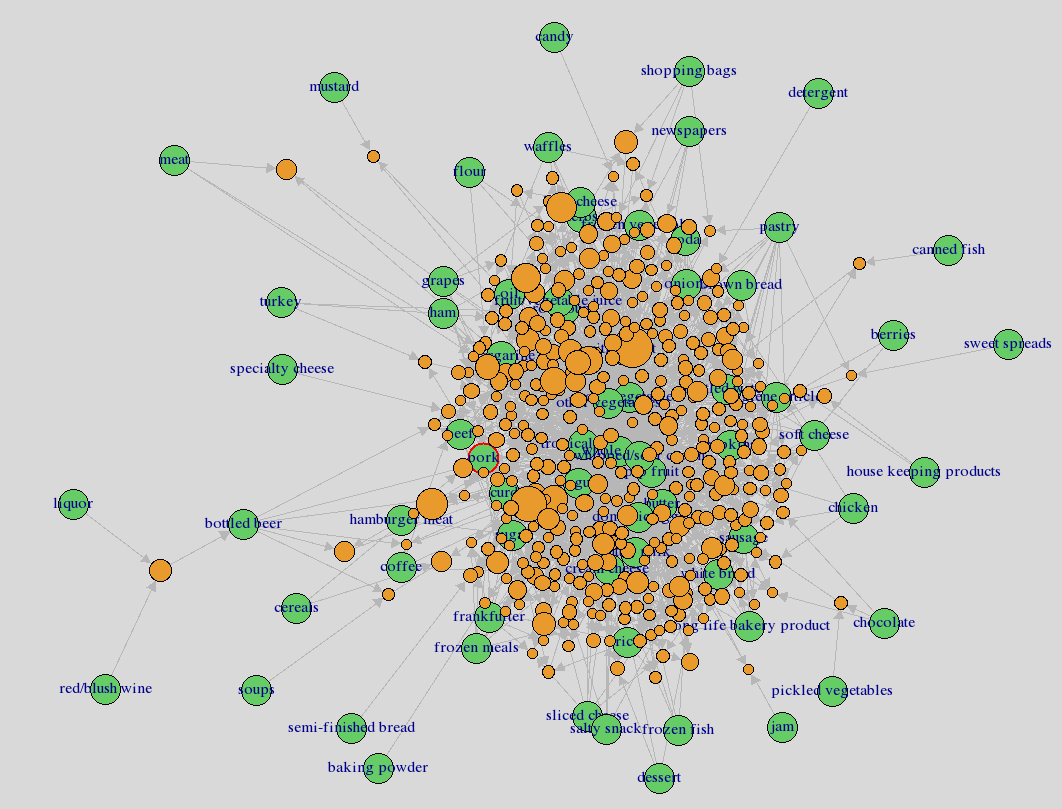
\includegraphics[width=14.75in]{figure/arulesViz}

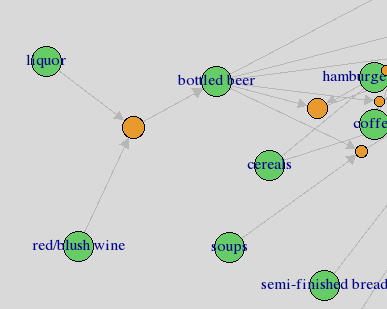
\includegraphics[width=5.38in]{figure/arulesVizBig}

\hypertarget{open-source-packages}{%
\section{Open Source Packages}\label{open-source-packages}}

\hypertarget{prophet}{%
\subsection{Prophet}\label{prophet}}

Prophet 是 Facebook在2017年開放出來的時序性預測演算法,用來預測各類資料的時序變化,像是顧客造訪數、溫度、疾病發生率等等,以下是Prophet for R的安裝使用範例

\begin{itemize}
\tightlist
\item
  C/C++ Tool

  \begin{itemize}
  \tightlist
  \item
    \href{https://cran.r-project.org/bin/windows/Rtools/}{R Tools} on Windows
  \item
    \href{http://osxdaily.com/2014/02/12/install-command-line-tools-mac-os-x/}{Command Line Tools} on OS X
  \end{itemize}
\end{itemize}

\begin{Shaded}
\begin{Highlighting}[]
\KeywordTok{install.packages}\NormalTok{(}\StringTok{'prophet'}\NormalTok{)}
\end{Highlighting}
\end{Shaded}

\href{https://facebookincubator.github.io/prophet/docs/quick_start.html\#r-api}{R API}

\begin{Shaded}
\begin{Highlighting}[]
\KeywordTok{library}\NormalTok{(prophet)}
\KeywordTok{library}\NormalTok{(dplyr)}
\NormalTok{df <-}\StringTok{ }\KeywordTok{read.csv}\NormalTok{(}\StringTok{'https://raw.githubusercontent.com/facebookincubator/prophet/master/examples/example_wp_peyton_manning.csv'}\NormalTok{) }\OperatorTok
\StringTok{    }\KeywordTok{mutate}\NormalTok{(}\DataTypeTok{y =} \KeywordTok{log}\NormalTok{(y))}
\NormalTok{m <-}\StringTok{ }\KeywordTok{prophet}\NormalTok{(df)}
\NormalTok{future <-}\StringTok{ }\KeywordTok{make_future_dataframe}\NormalTok{(m, }\DataTypeTok{periods =} \DecValTok{365}\NormalTok{)}
\KeywordTok{tail}\NormalTok{(future)}
\NormalTok{forecast <-}\StringTok{ }\KeywordTok{predict}\NormalTok{(m, future)}
\KeywordTok{tail}\NormalTok{(forecast[}\KeywordTok{c}\NormalTok{(}\StringTok{'ds'}\NormalTok{, }\StringTok{'yhat'}\NormalTok{, }\StringTok{'yhat_lower'}\NormalTok{, }\StringTok{'yhat_upper'}\NormalTok{)])}
\KeywordTok{plot}\NormalTok{(m, forecast)}
\KeywordTok{prophet_plot_components}\NormalTok{(m, forecast)}
\end{Highlighting}
\end{Shaded}

\href{https://facebookincubator.github.io/prophet/}{Prophet官網}

\hypertarget{tensorflow}{%
\subsection{TensorFlow}\label{tensorflow}}

\begin{itemize}
\tightlist
\item
  Python 3.5.3 \textbf{64 bit} \href{https://www.python.org/downloads/release/python-353/}{網站}

  \begin{itemize}
  \tightlist
  \item
    Windows x86-64 executable installer
  \end{itemize}
\item
  TensorFlow 1.0.1 \href{https://www.tensorflow.org/install/}{網站}

  \begin{itemize}
  \tightlist
  \item
    pip3 install --upgrade tensorflow
  \item
    pip3 install --upgrade tensorflow-gpu
  \end{itemize}
\item
  C/C++ Tool

  \begin{itemize}
  \tightlist
  \item
    \href{https://cran.r-project.org/bin/windows/Rtools/}{R Tools} on Windows
  \item
    \href{http://osxdaily.com/2014/02/12/install-command-line-tools-mac-os-x/}{Command Line Tools} on OS X
  \end{itemize}
\item
  tensorflow package for R \href{https://rstudio.github.io/tensorflow/index.html}{網站}
\end{itemize}

\begin{Shaded}
\begin{Highlighting}[]
\NormalTok{devtools}\OperatorTok{::}\KeywordTok{install_github}\NormalTok{(}\StringTok{"rstudio/tensorflow"}\NormalTok{)}
\end{Highlighting}
\end{Shaded}

TensorFlow for R

\begin{itemize}
\tightlist
\item
  Locating TensorFlow (optional)
\item
  Hello World
\end{itemize}

\begin{Shaded}
\begin{Highlighting}[]
\KeywordTok{library}\NormalTok{(tensorflow)}
\NormalTok{sess =}\StringTok{ }\NormalTok{tf}\OperatorTok{$}\KeywordTok{Session}\NormalTok{()}
\NormalTok{hello <-}\StringTok{ }\NormalTok{tf}\OperatorTok{$}\KeywordTok{constant}\NormalTok{(}\StringTok{'Hello, TensorFlow!'}\NormalTok{)}
\NormalTok{sess}\OperatorTok{$}\KeywordTok{run}\NormalTok{(hello)}
\end{Highlighting}
\end{Shaded}

\hypertarget{mxnet}{%
\subsection{MXNet}\label{mxnet}}

Amazon
\href{http://mxnet.io/get_started/windows_setup.html\#install-mxnet-for-r}{Install MXNet for R}
MXNet for R \href{http://mxnet.io/tutorials/index.html\#r}{Tutorials}

MXNet for R

\begin{Shaded}
\begin{Highlighting}[]
\KeywordTok{install.packages}\NormalTok{(}\StringTok{"drat"}\NormalTok{, }\DataTypeTok{repos=}\StringTok{"https://cran.rstudio.com"}\NormalTok{)}
\NormalTok{drat}\OperatorTok{:::}\KeywordTok{addRepo}\NormalTok{(}\StringTok{"dmlc"}\NormalTok{)}
\KeywordTok{install.packages}\NormalTok{(}\StringTok{"mxnet"}\NormalTok{)}
\end{Highlighting}
\end{Shaded}

\hypertarget{ux6a21ux578bux9a57ux8b49}{%
\section{模型驗證}\label{ux6a21ux578bux9a57ux8b49}}

在完成模型訓練後,為了驗證模型訓練的好不好,需要用一組\textbf{獨立}的測試資料,來做模型的驗證。所以,在訓練模型前,必須特別留意是否有保留一份\textbf{獨立的資料},並確保在訓練模型時都不用到此獨立資料集。因此,資料集可分為以下兩種:

\begin{itemize}
\tightlist
\item
  \textbf{訓練組} Training set, Development set: 讓演算法\texttt{學}到\texttt{知識}
\item
  \textbf{測試組} Test set, Validation set: 驗證\texttt{學}的怎麼樣
\end{itemize}

Training set和Test set通常會比例分配,如2/3的資料設為\texttt{Training\ set},剩下的1/3做驗證\texttt{Test\ set}。以下圖的監督式學習流程圖為例,可以注意到綠色箭頭的資料集在訓練過程中從未被使用。

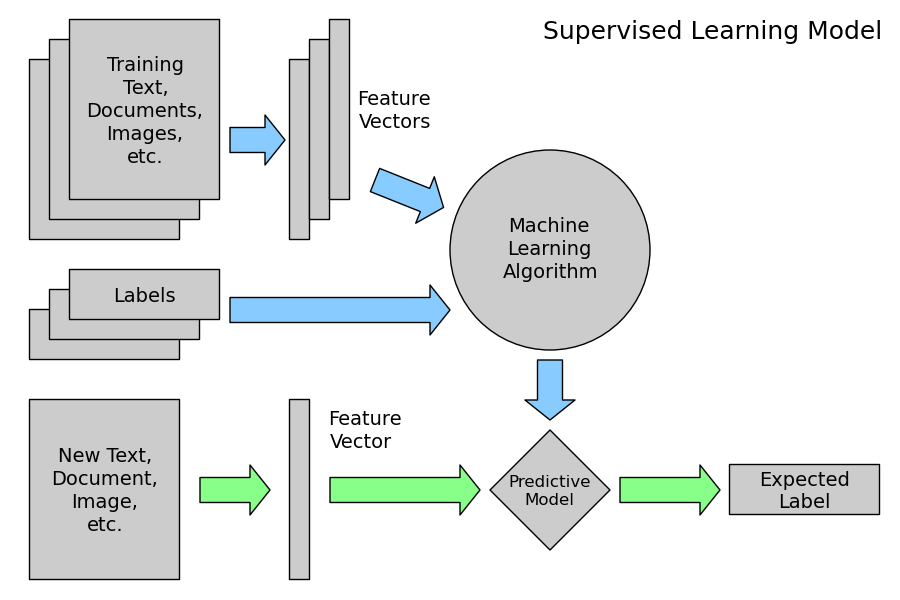
\includegraphics[width=12.5in]{figure/SupervisedLearning}

\hypertarget{regression-ux8ff4ux6b78ux9a57ux8b49}{%
\subsection{Regression 迴歸驗證}\label{regression-ux8ff4ux6b78ux9a57ux8b49}}

以NBA資料為例,首先先將資料讀入

\begin{Shaded}
\begin{Highlighting}[]
\CommentTok{#讀入SportsAnalytics package}
\ControlFlowTok{if}\NormalTok{ (}\OperatorTok{!}\KeywordTok{require}\NormalTok{(}\StringTok{'SportsAnalytics'}\NormalTok{))\{}
    \KeywordTok{install.packages}\NormalTok{(}\StringTok{"SportsAnalytics"}\NormalTok{)}
    \KeywordTok{library}\NormalTok{(SportsAnalytics)}
\NormalTok{\}}
\CommentTok{#擷取2015-2016年球季球員資料}
\NormalTok{NBA1516<-}\KeywordTok{fetch_NBAPlayerStatistics}\NormalTok{(}\StringTok{"15-16"}\NormalTok{)}
\NormalTok{NBA1516<-NBA1516[}\KeywordTok{complete.cases}\NormalTok{(NBA1516),]}
\end{Highlighting}
\end{Shaded}

\begin{itemize}
\tightlist
\item
  以Training set來\texttt{選看起來最好的模型}
\item
  用Test set來\texttt{驗證模型是不是真的很好}
\item
  想像\ldots..訓練出來題庫答得好的學生,寫到新題目不一定會寫!?
\item
  訓練模型時,只能看Training set,用Training set來選一個最好的模型
\item
  訓練模型時,不能偷看Test set,才是真正的驗證
\end{itemize}

為分出訓練組與測試組,需使用隨機抽樣的方式

\begin{Shaded}
\begin{Highlighting}[]
\KeywordTok{sample}\NormalTok{(}\DecValTok{1}\OperatorTok{:}\DecValTok{10}\NormalTok{,}\DecValTok{3}\NormalTok{) }\CommentTok{# 從1到10,隨機取三個數字}
\end{Highlighting}
\end{Shaded}

\begin{verbatim}
## [1] 8 3 4
\end{verbatim}

\begin{Shaded}
\begin{Highlighting}[]
\KeywordTok{sample}\NormalTok{(}\DecValTok{1}\OperatorTok{:}\KeywordTok{nrow}\NormalTok{(NBA1516),}\KeywordTok{nrow}\NormalTok{(NBA1516)}\OperatorTok{/}\DecValTok{3}\NormalTok{) }\CommentTok{#從第一行到最後一行,隨機取1/3行數}
\end{Highlighting}
\end{Shaded}

\begin{verbatim}
##   [1]  93 122 389  66 175 424 379 468 304 108 131 343  41 115 228 328 416
##  [18] 298 299 258 117  79 182 305 358 184 307 390 452 221 224  49 313 136
##  [35] 282 145 123 264 234  96  22 291 297 208 465 342  57  10 406 248 365
##  [52] 153 431  83 245 426 218 215 326 276 169  71  61 352 417 383 155 460
##  [69] 467  60  36 375  19 137 126 158 319 116 440 102 214 314 448  85 392
##  [86] 160  77  17 401 262 130 181 267 316 356 163 461 277 396 134 265 403
## [103] 249 435  40  29 425 185 294  88 400 363 411 335  86 142 147 414 188
## [120] 355  26 372 418  28 101 296 323 408 359 189 196  84 422 250 388 281
## [137] 380 471  30 428 354 444  80  73 148  12 293 195 303 361 166 347 146
## [154] 107 240  31   6 263
\end{verbatim}

使用上述方法,選出1/3的元素位置,把NBA的資料分成Training 和 Test set

\begin{Shaded}
\begin{Highlighting}[]
\NormalTok{NBA1516}\OperatorTok{$}\NormalTok{Test<-F }\CommentTok{#新增一個參數紀錄分組}
\CommentTok{#隨機取1/3當Test set}
\NormalTok{NBA1516[}\KeywordTok{sample}\NormalTok{(}\DecValTok{1}\OperatorTok{:}\KeywordTok{nrow}\NormalTok{(NBA1516),}\KeywordTok{nrow}\NormalTok{(NBA1516)}\OperatorTok{/}\DecValTok{3}\NormalTok{),]}\OperatorTok{$}\NormalTok{Test<-T}
\CommentTok{# Training set : Test set球員數}
\KeywordTok{c}\NormalTok{(}\KeywordTok{sum}\NormalTok{(NBA1516}\OperatorTok{$}\NormalTok{Test}\OperatorTok{==}\NormalTok{F),}\KeywordTok{sum}\NormalTok{(NBA1516}\OperatorTok{$}\NormalTok{Test}\OperatorTok{==}\NormalTok{T))}
\end{Highlighting}
\end{Shaded}

\begin{verbatim}
## [1] 317 158
\end{verbatim}

並用訓練組的資料(NBA1516\$Test==F),訓練一個多變數線性迴歸模型

\begin{Shaded}
\begin{Highlighting}[]
\NormalTok{fit<-}\KeywordTok{glm}\NormalTok{(TotalPoints}\OperatorTok{~}\NormalTok{TotalMinutesPlayed}\OperatorTok{+}\NormalTok{FieldGoalsAttempted}\OperatorTok{+}
\StringTok{             }\NormalTok{Position}\OperatorTok{+}\NormalTok{ThreesAttempted}\OperatorTok{+}\NormalTok{FreeThrowsAttempted,}
              \DataTypeTok{data =}\NormalTok{NBA1516[NBA1516}\OperatorTok{$}\NormalTok{Test}\OperatorTok{==}\NormalTok{F,])}
\KeywordTok{summary}\NormalTok{(fit)}\OperatorTok{$}\NormalTok{coefficients}
\end{Highlighting}
\end{Shaded}

\begin{verbatim}
##                     Estimate Std. Error t value Pr(>|t|)
## (Intercept)          1.5e+01     7.1299   2.142  3.3e-02
## TotalMinutesPlayed   2.4e-04     0.0067   0.036  9.7e-01
## FieldGoalsAttempted  1.0e+00     0.0205  49.638 5.4e-149
## PositionPF          -2.1e+01     7.2007  -2.852  4.6e-03
## PositionPG          -4.4e+01     7.8172  -5.680  3.1e-08
## PositionSF          -3.0e+01     8.1923  -3.688  2.7e-04
## PositionSG          -3.2e+01     8.0354  -3.947  9.8e-05
## ThreesAttempted      9.5e-02     0.0261   3.630  3.3e-04
## FreeThrowsAttempted  7.2e-01     0.0357  20.161  3.2e-58
\end{verbatim}

逐步選擇模型 stepwise 後退學習:一開始先將所有參數加到模型裡,再一個一個拿掉

\begin{Shaded}
\begin{Highlighting}[]
\KeywordTok{library}\NormalTok{(MASS)}
\CommentTok{##根據AIC,做逐步選擇, 預設倒退學習 direction = "backward"}
\CommentTok{##trace=FALSE: 不要顯示步驟}
\NormalTok{finalModel_B<-}\KeywordTok{stepAIC}\NormalTok{(fit,}\DataTypeTok{direction =} \StringTok{"backward"}\NormalTok{,}\DataTypeTok{trace=}\OtherTok{FALSE}\NormalTok{)}
\KeywordTok{summary}\NormalTok{(finalModel_B)}\OperatorTok{$}\NormalTok{coefficients}
\end{Highlighting}
\end{Shaded}

\begin{verbatim}
##                     Estimate Std. Error t value Pr(>|t|)
## (Intercept)           15.379      6.489     2.4  1.8e-02
## FieldGoalsAttempted    1.017      0.015    67.4 7.2e-187
## PositionPF           -20.570      7.127    -2.9  4.2e-03
## PositionPG           -44.451      7.697    -5.8  1.9e-08
## PositionSF           -30.230      8.168    -3.7  2.5e-04
## PositionSG           -31.761      7.933    -4.0  7.8e-05
## ThreesAttempted        0.095      0.026     3.7  3.0e-04
## FreeThrowsAttempted    0.719      0.036    20.2  2.1e-58
\end{verbatim}

逐步選擇模型 stepwise 往前學習:一開始先做一個沒有參數的模型,再把參數一個一個加進去

\begin{Shaded}
\begin{Highlighting}[]
\CommentTok{##根據AIC,做逐步選擇, 往前學習 direction = "forward"}
\NormalTok{finalModel_F<-}\KeywordTok{stepAIC}\NormalTok{(fit,}\DataTypeTok{direction =} \StringTok{"forward"}\NormalTok{,}\DataTypeTok{trace=}\OtherTok{FALSE}\NormalTok{)}
\KeywordTok{summary}\NormalTok{(finalModel_F)}\OperatorTok{$}\NormalTok{coefficients}
\end{Highlighting}
\end{Shaded}

\begin{verbatim}
##                     Estimate Std. Error t value Pr(>|t|)
## (Intercept)          1.5e+01     7.1299   2.142  3.3e-02
## TotalMinutesPlayed   2.4e-04     0.0067   0.036  9.7e-01
## FieldGoalsAttempted  1.0e+00     0.0205  49.638 5.4e-149
## PositionPF          -2.1e+01     7.2007  -2.852  4.6e-03
## PositionPG          -4.4e+01     7.8172  -5.680  3.1e-08
## PositionSF          -3.0e+01     8.1923  -3.688  2.7e-04
## PositionSG          -3.2e+01     8.0354  -3.947  9.8e-05
## ThreesAttempted      9.5e-02     0.0261   3.630  3.3e-04
## FreeThrowsAttempted  7.2e-01     0.0357  20.161  3.2e-58
\end{verbatim}

逐步選擇模型 stepwise 雙向學習:參數加加減減

\begin{Shaded}
\begin{Highlighting}[]
\CommentTok{##根據AIC,做逐步選擇, 雙向學習 direction = "both"}
\NormalTok{finalModel_Both<-}\KeywordTok{stepAIC}\NormalTok{(fit,}\DataTypeTok{direction =} \StringTok{"both"}\NormalTok{,}\DataTypeTok{trace=}\OtherTok{FALSE}\NormalTok{)}
\KeywordTok{summary}\NormalTok{(finalModel_Both)}\OperatorTok{$}\NormalTok{coefficients}
\end{Highlighting}
\end{Shaded}

\begin{verbatim}
##                     Estimate Std. Error t value Pr(>|t|)
## (Intercept)           15.379      6.489     2.4  1.8e-02
## FieldGoalsAttempted    1.017      0.015    67.4 7.2e-187
## PositionPF           -20.570      7.127    -2.9  4.2e-03
## PositionPG           -44.451      7.697    -5.8  1.9e-08
## PositionSF           -30.230      8.168    -3.7  2.5e-04
## PositionSG           -31.761      7.933    -4.0  7.8e-05
## ThreesAttempted        0.095      0.026     3.7  3.0e-04
## FreeThrowsAttempted    0.719      0.036    20.2  2.1e-58
\end{verbatim}

用Test set來評估模型好不好,使用predict函數,將測試組資料放入預測模型中,預測測試組的結果

\begin{Shaded}
\begin{Highlighting}[]
\NormalTok{predictPoint<-}\KeywordTok{predict}\NormalTok{(finalModel_Both, }\CommentTok{#Test==T, test data}
                      \DataTypeTok{newdata =}\NormalTok{ NBA1516[NBA1516}\OperatorTok{$}\NormalTok{Test}\OperatorTok{==}\NormalTok{T,])}
\KeywordTok{cor}\NormalTok{(}\DataTypeTok{x=}\NormalTok{predictPoint,}\DataTypeTok{y=}\NormalTok{NBA1516[NBA1516}\OperatorTok{$}\NormalTok{Test}\OperatorTok{==}\NormalTok{T,]}\OperatorTok{$}\NormalTok{TotalPoints) }\CommentTok{#相關係數}
\end{Highlighting}
\end{Shaded}

\begin{verbatim}
## [1] 1
\end{verbatim}

\begin{Shaded}
\begin{Highlighting}[]
\KeywordTok{plot}\NormalTok{(}\DataTypeTok{x=}\NormalTok{predictPoint,}\DataTypeTok{y=}\NormalTok{NBA1516[NBA1516}\OperatorTok{$}\NormalTok{Test}\OperatorTok{==}\NormalTok{T,]}\OperatorTok{$}\NormalTok{TotalPoints)}
\end{Highlighting}
\end{Shaded}

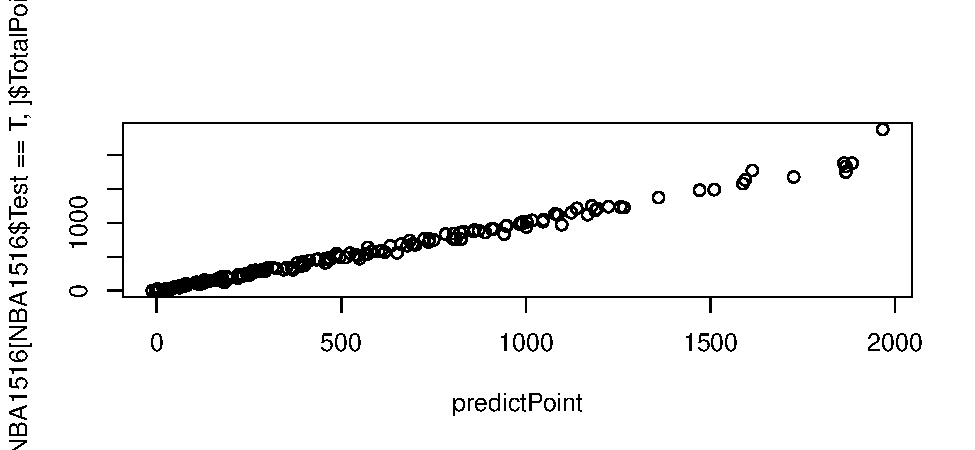
\includegraphics{DataAnalyticsWithR_files/figure-latex/unnamed-chunk-50-1.pdf}

\hypertarget{logistic-regression-ux908fux8f2fux8ff4ux6b78ux9a57ux8b49}{%
\subsection{Logistic Regression 邏輯迴歸驗證}\label{logistic-regression-ux908fux8f2fux8ff4ux6b78ux9a57ux8b49}}

首先,先把入學資料分成Training 和 Test set。這邊要特別留意,當答案有正反兩面時,\texttt{Level\ 1\ 要放正面答案}--\textgreater 有病/錄取\ldots{}

\begin{Shaded}
\begin{Highlighting}[]
\NormalTok{mydata <-}\StringTok{ }\KeywordTok{read.csv}\NormalTok{(}\StringTok{"https://raw.githubusercontent.com/CGUIM-BigDataAnalysis/BigDataCGUIM/master/binary.csv"}\NormalTok{)}
\NormalTok{mydata}\OperatorTok{$}\NormalTok{admit <-}\StringTok{ }\KeywordTok{factor}\NormalTok{(mydata}\OperatorTok{$}\NormalTok{admit) }\CommentTok{# 類別變項要轉為factor}
\NormalTok{mydata}\OperatorTok{$}\NormalTok{rank <-}\StringTok{ }\KeywordTok{factor}\NormalTok{(mydata}\OperatorTok{$}\NormalTok{rank) }\CommentTok{# 類別變項要轉為factor}
\NormalTok{mydata}\OperatorTok{$}\NormalTok{Test<-F }\CommentTok{#新增一個參數紀錄分組}
\NormalTok{mydata[}\KeywordTok{sample}\NormalTok{(}\DecValTok{1}\OperatorTok{:}\KeywordTok{nrow}\NormalTok{(mydata),}\KeywordTok{nrow}\NormalTok{(mydata)}\OperatorTok{/}\DecValTok{3}\NormalTok{),]}\OperatorTok{$}\NormalTok{Test<-T }\CommentTok{#隨機取1/3當Test set}
\KeywordTok{c}\NormalTok{(}\KeywordTok{sum}\NormalTok{(mydata}\OperatorTok{$}\NormalTok{Test}\OperatorTok{==}\NormalTok{F),}\KeywordTok{sum}\NormalTok{(mydata}\OperatorTok{$}\NormalTok{Test}\OperatorTok{==}\NormalTok{T)) }\CommentTok{# Training set : Test set學生數}
\end{Highlighting}
\end{Shaded}

\begin{verbatim}
## [1] 267 133
\end{verbatim}

\begin{Shaded}
\begin{Highlighting}[]
\CommentTok{#修改一下factor的level: 改成Level 1為錄取,2為不錄取-->Level 1 要放正面答案}
\NormalTok{mydata}\OperatorTok{$}\NormalTok{admit<-}\KeywordTok{factor}\NormalTok{(mydata}\OperatorTok{$}\NormalTok{admit,}\DataTypeTok{levels=}\KeywordTok{c}\NormalTok{(}\DecValTok{1}\NormalTok{,}\DecValTok{0}\NormalTok{))}
\end{Highlighting}
\end{Shaded}

逐步選擇最好的模型

\begin{Shaded}
\begin{Highlighting}[]
\CommentTok{# GRE:某考試成績, GPA:在校平均成績, rank:學校聲望}
\NormalTok{mylogit <-}\StringTok{ }\KeywordTok{glm}\NormalTok{(admit }\OperatorTok{~}\StringTok{ }\NormalTok{gre }\OperatorTok{+}\StringTok{ }\NormalTok{gpa }\OperatorTok{+}\StringTok{ }\NormalTok{rank,}
               \DataTypeTok{data =}\NormalTok{ mydata[mydata}\OperatorTok{$}\NormalTok{Test}\OperatorTok{==}\NormalTok{F,], }\DataTypeTok{family =} \StringTok{"binomial"}\NormalTok{)}
\NormalTok{finalFit<-}\KeywordTok{stepAIC}\NormalTok{(mylogit,}\DataTypeTok{direction =} \StringTok{"both"}\NormalTok{,}\DataTypeTok{trace=}\OtherTok{FALSE}\NormalTok{) }\CommentTok{# 雙向逐步選擇模型}
\KeywordTok{summary}\NormalTok{(finalFit)}
\end{Highlighting}
\end{Shaded}

\begin{verbatim}
## 
## Call:
## glm(formula = admit ~ gpa + rank, family = "binomial", data = mydata[mydata$Test == 
##     F, ])
## 
## Deviance Residuals: 
##    Min      1Q  Median      3Q     Max  
## -2.174  -1.145   0.656   0.892   1.450  
## 
## Coefficients:
##             Estimate Std. Error z value Pr(>|z|)   
## (Intercept)    4.017      1.404    2.86   0.0042 **
## gpa           -1.160      0.388   -2.99   0.0028 **
## rank2          0.487      0.400    1.22   0.2235   
## rank3          1.064      0.420    2.53   0.0114 * 
## rank4          1.563      0.536    2.91   0.0036 **
## ---
## Signif. codes:  0 '***' 0.001 '**' 0.01 '*' 0.05 '.' 0.1 ' ' 1
## 
## (Dispersion parameter for binomial family taken to be 1)
## 
##     Null deviance: 332.54  on 266  degrees of freedom
## Residual deviance: 308.28  on 262  degrees of freedom
## AIC: 318.3
## 
## Number of Fisher Scoring iterations: 4
\end{verbatim}

用預測組預測新學生可不可以錄取,並驗證答案

\begin{Shaded}
\begin{Highlighting}[]
\NormalTok{AdmitProb<-}\KeywordTok{predict}\NormalTok{(finalFit, }\CommentTok{# 用Training set做的模型}
                   \DataTypeTok{newdata =}\NormalTok{ mydata[mydata}\OperatorTok{$}\NormalTok{Test}\OperatorTok{==}\NormalTok{T,], }\CommentTok{#Test==T, test data}
                   \DataTypeTok{type=}\StringTok{"response"}\NormalTok{) }\CommentTok{#結果為每個人被錄取的機率}
\KeywordTok{head}\NormalTok{(AdmitProb)}
\end{Highlighting}
\end{Shaded}

\begin{verbatim}
##    3    6    7   11   12   14 
## 0.65 0.63 0.49 0.61 0.77 0.85
\end{verbatim}

\begin{Shaded}
\begin{Highlighting}[]
\KeywordTok{table}\NormalTok{(AdmitProb}\OperatorTok{<}\FloatTok{0.5}\NormalTok{,mydata[mydata}\OperatorTok{$}\NormalTok{Test}\OperatorTok{==}\NormalTok{T,]}\OperatorTok{$}\NormalTok{admit) }\CommentTok{# row,column}
\end{Highlighting}
\end{Shaded}

\begin{verbatim}
##        
##          1  0
##   FALSE 35 88
##   TRUE   6  4
\end{verbatim}

當答案是二元時:效能指標

\begin{itemize}
\tightlist
\item
  Sensitivity 敏感性
\item
  Specificity 特異性
\item
  Positive Predictive Value (PPV) 陽性預測值
\item
  Negative Predictive Value (NPV) 陰性預測值
\end{itemize}

名詞解釋

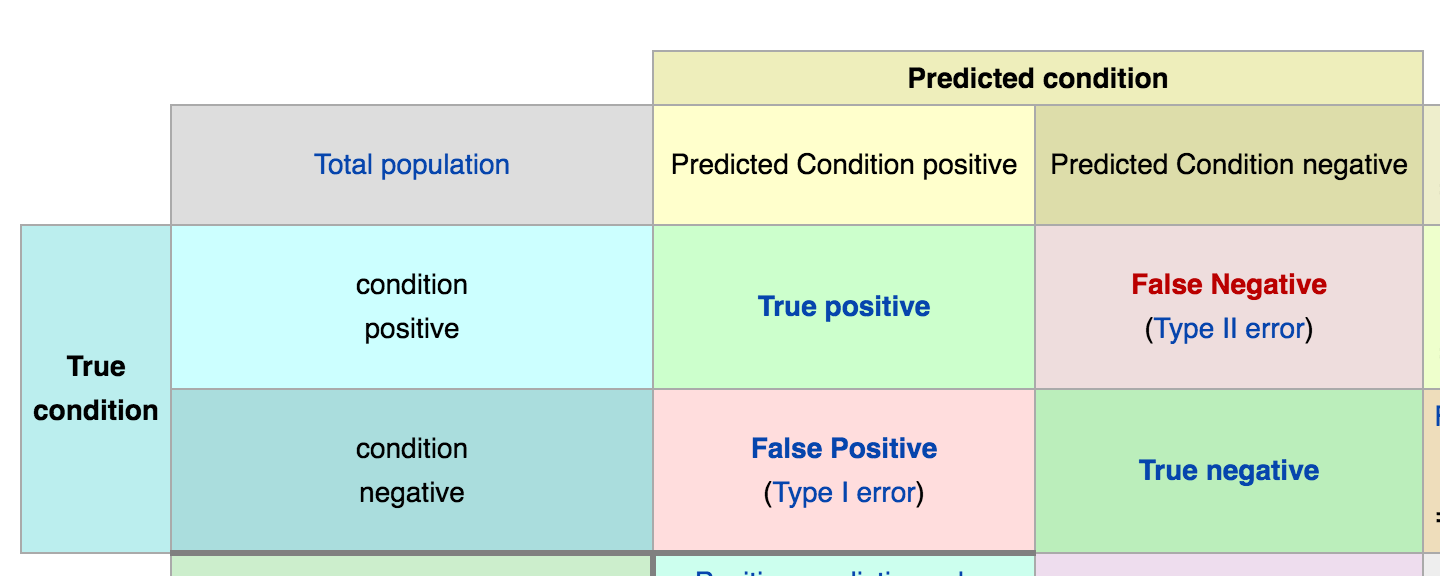
\includegraphics[width=20in]{figure/Cond}

\begin{itemize}
\tightlist
\item
  TP: 有病且預測也有病
\item
  TN: 沒病且預測也沒病
\item
  FP: 沒病但是預測有病
\item
  FN: 有病但預測沒病
\end{itemize}

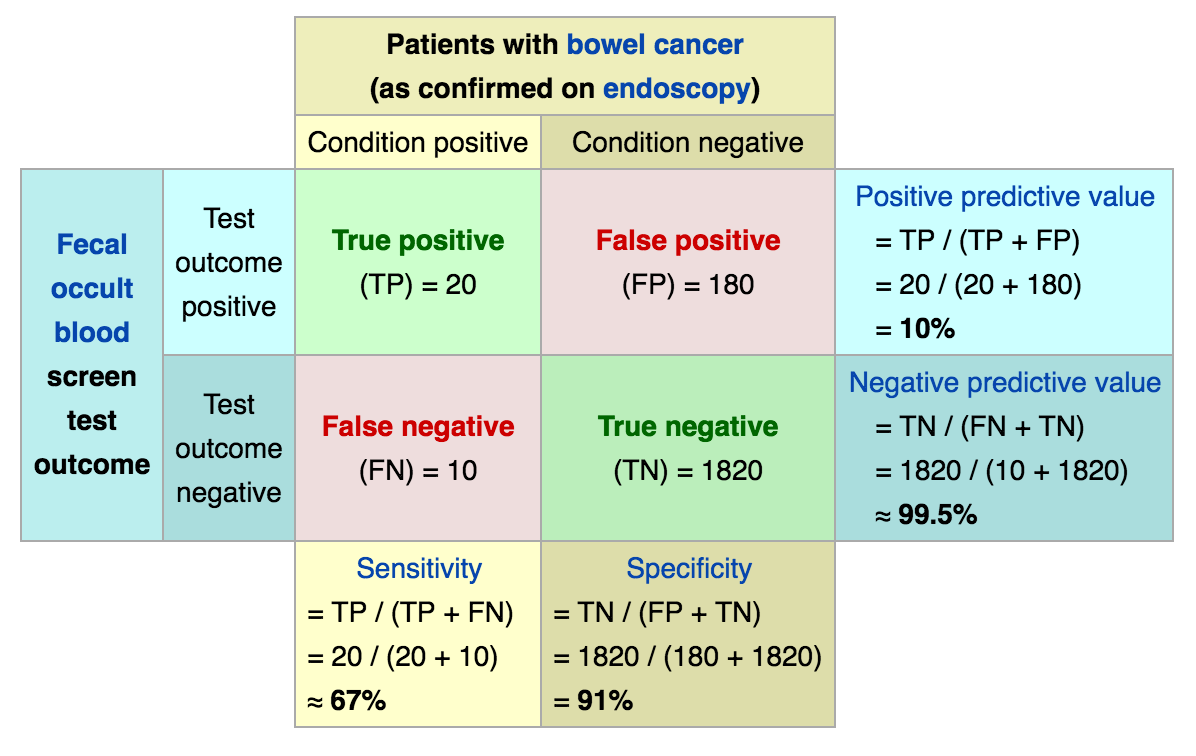
\includegraphics[width=16.61in]{figure/para}

當答案是二元時:效能指標公式

\begin{itemize}
\tightlist
\item
  Sensitivity 敏感性:所有\texttt{真的有病}的人,被\texttt{預測有病}的比例
\item
  Specificity 特異性:所有\texttt{真的沒病}的人,被\texttt{預測沒病}的比例
\item
  Positive Predictive Value (PPV) 陽性預測值:所有被\texttt{預測有病}的人,\texttt{真的有病}的比例
\item
  Negative Predictive Value (NPV) 陰性預測值:所有被\texttt{預測沒病}的人,\texttt{真的沒病}的比例
\end{itemize}

回想一下剛剛的驗證結果

\begin{Shaded}
\begin{Highlighting}[]
\KeywordTok{table}\NormalTok{(AdmitProb}\OperatorTok{<}\FloatTok{0.5}\NormalTok{,mydata[mydata}\OperatorTok{$}\NormalTok{Test}\OperatorTok{==}\NormalTok{T,]}\OperatorTok{$}\NormalTok{admit) }\CommentTok{# row,column}
\end{Highlighting}
\end{Shaded}

\begin{verbatim}
##        
##          1  0
##   FALSE 35 88
##   TRUE   6  4
\end{verbatim}

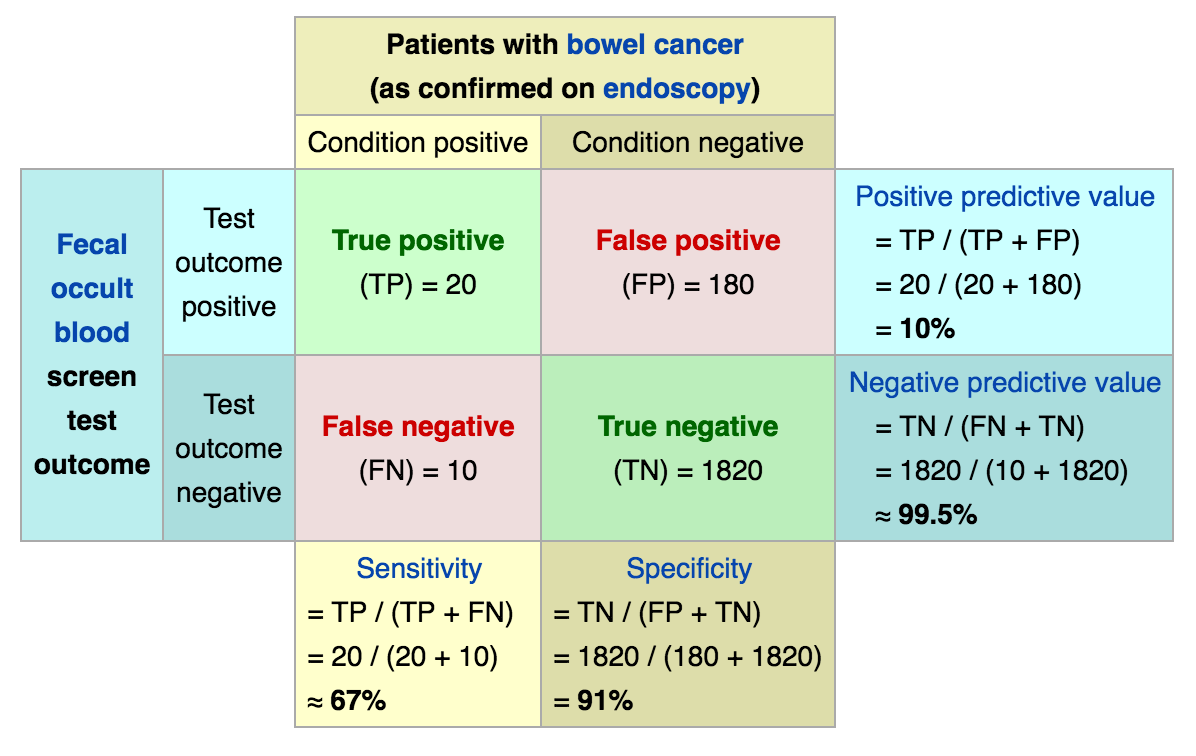
\includegraphics[width=16.61in]{figure/para}

計算預測效能參數

\begin{Shaded}
\begin{Highlighting}[]
\NormalTok{AdmitProb<-}\KeywordTok{predict}\NormalTok{(finalFit,}
                   \DataTypeTok{newdata =}\NormalTok{ mydata[mydata}\OperatorTok{$}\NormalTok{Test}\OperatorTok{==}\NormalTok{T,], }\CommentTok{#Test==T, test data}
                   \DataTypeTok{type=}\StringTok{"response"}\NormalTok{) }\CommentTok{#結果為每個人『不』被錄取的機率}
\NormalTok{AdmitAns<-}\KeywordTok{factor}\NormalTok{(}\KeywordTok{ifelse}\NormalTok{(AdmitProb}\OperatorTok{<}\FloatTok{0.5}\NormalTok{,}\DecValTok{1}\NormalTok{,}\DecValTok{0}\NormalTok{),}\DataTypeTok{levels=}\KeywordTok{c}\NormalTok{(}\DecValTok{1}\NormalTok{,}\DecValTok{0}\NormalTok{))}
\KeywordTok{str}\NormalTok{(AdmitAns)}
\end{Highlighting}
\end{Shaded}

\begin{verbatim}
##  Factor w/ 2 levels "1","0": 2 2 1 2 2 2 2 2 2 2 ...
##  - attr(*, "names")= chr [1:133] "3" "6" "7" "11" ...
\end{verbatim}

計算預測效能參數

\begin{Shaded}
\begin{Highlighting}[]
\KeywordTok{library}\NormalTok{(caret) }\CommentTok{# install.packages("caret") #計算參數的packages}
\KeywordTok{sensitivity}\NormalTok{(AdmitAns,mydata[mydata}\OperatorTok{$}\NormalTok{Test}\OperatorTok{==}\NormalTok{T,]}\OperatorTok{$}\NormalTok{admit)}
\end{Highlighting}
\end{Shaded}

\begin{verbatim}
## [1] 0.15
\end{verbatim}

\begin{Shaded}
\begin{Highlighting}[]
\KeywordTok{specificity}\NormalTok{(AdmitAns,mydata[mydata}\OperatorTok{$}\NormalTok{Test}\OperatorTok{==}\NormalTok{T,]}\OperatorTok{$}\NormalTok{admit)}
\end{Highlighting}
\end{Shaded}

\begin{verbatim}
## [1] 0.96
\end{verbatim}

\begin{Shaded}
\begin{Highlighting}[]
\KeywordTok{posPredValue}\NormalTok{(AdmitAns,mydata[mydata}\OperatorTok{$}\NormalTok{Test}\OperatorTok{==}\NormalTok{T,]}\OperatorTok{$}\NormalTok{admit)}
\end{Highlighting}
\end{Shaded}

\begin{verbatim}
## [1] 0.6
\end{verbatim}

\begin{Shaded}
\begin{Highlighting}[]
\KeywordTok{negPredValue}\NormalTok{(AdmitAns,mydata[mydata}\OperatorTok{$}\NormalTok{Test}\OperatorTok{==}\NormalTok{T,]}\OperatorTok{$}\NormalTok{admit)}
\end{Highlighting}
\end{Shaded}

\begin{verbatim}
## [1] 0.72
\end{verbatim}

\hypertarget{decision-trees-ux6c7aux7b56ux6a39ux9a57ux8b49}{%
\subsection{Decision Trees 決策樹驗證}\label{decision-trees-ux6c7aux7b56ux6a39ux9a57ux8b49}}

阻攻/籃板/三分/助攻/抄截判斷位置-訓練

\begin{Shaded}
\begin{Highlighting}[]
\ControlFlowTok{if}\NormalTok{ (}\OperatorTok{!}\KeywordTok{require}\NormalTok{(}\StringTok{'rpart'}\NormalTok{))\{}
    \KeywordTok{install.packages}\NormalTok{(}\StringTok{"rpart"}\NormalTok{); }\KeywordTok{library}\NormalTok{(rpart)}
\NormalTok{\}}
\NormalTok{DT<-}\KeywordTok{rpart}\NormalTok{(Position}\OperatorTok{~}\NormalTok{Blocks}\OperatorTok{+}\NormalTok{TotalRebounds}\OperatorTok{+}\NormalTok{ThreesMade}\OperatorTok{+}\NormalTok{Assists}\OperatorTok{+}\NormalTok{Steals,}
          \DataTypeTok{data=}\NormalTok{NBA1516[NBA1516}\OperatorTok{$}\NormalTok{Test}\OperatorTok{==}\NormalTok{F,]) }\CommentTok{#訓練組 Training set}
\CommentTok{#控球後衛(PG)、得分後衛(SG)、小前鋒(SF)、大前鋒(PF)和中鋒(C)}
\NormalTok{DT}
\end{Highlighting}
\end{Shaded}

\begin{verbatim}
## n= 317 
## 
## node), split, n, loss, yval, (yprob)
##       * denotes terminal node
## 
##   1) root 317 240 PF (0.13 0.25 0.23 0.17 0.22)  
##     2) ThreesMade< 0.5 61  31 PF (0.43 0.49 0.033 0.049 0)  
##       4) TotalRebounds>=7.5 54  26 PF (0.48 0.52 0 0 0)  
##         8) TotalRebounds>=2.2e+02 28  11 C (0.61 0.39 0 0 0)  
##          16) Assists< 72 14   2 C (0.86 0.14 0 0 0) *
##          17) Assists>=72 14   5 PF (0.36 0.64 0 0 0) *
##         9) TotalRebounds< 2.2e+02 26   9 PF (0.35 0.65 0 0 0) *
##       5) TotalRebounds< 7.5 7   4 SF (0 0.29 0.29 0.43 0) *
##     3) ThreesMade>=0.5 256 180 SG (0.059 0.2 0.27 0.2 0.28)  
##       6) Assists>=1.7e+02 65  24 PG (0.046 0.031 0.63 0.12 0.17)  
##        12) TotalRebounds< 3.3e+02 43   7 PG (0.023 0 0.84 0.047 0.093) *
##        13) TotalRebounds>=3.3e+02 22  15 SG (0.091 0.091 0.23 0.27 0.32)  
##          26) Assists>=3.8e+02 7   2 PG (0 0 0.71 0.29 0) *
##          27) Assists< 3.8e+02 15   8 SG (0.13 0.13 0 0.27 0.47) *
##       7) Assists< 1.7e+02 191 130 SG (0.063 0.25 0.15 0.22 0.31)  
##        14) TotalRebounds>=2.8e+02 47  23 PF (0.19 0.51 0 0.28 0.021)  
##          28) Steals< 64 35  12 PF (0.2 0.66 0 0.11 0.029) *
##          29) Steals>=64 12   3 SF (0.17 0.083 0 0.75 0) *
##        15) TotalRebounds< 2.8e+02 144  85 SG (0.021 0.17 0.2 0.2 0.41)  
##          30) Blocks>=6.5 84  48 SG (0.024 0.25 0.071 0.23 0.43)  
##            60) ThreesMade< 14 17   5 PF (0 0.71 0 0.29 0) *
##            61) ThreesMade>=14 67  31 SG (0.03 0.13 0.09 0.21 0.54)  
##             122) Steals< 35 33  20 SG (0.03 0.27 0.03 0.27 0.39)  
##               244) TotalRebounds>=2e+02 8   2 PF (0.12 0.75 0 0 0.12) *
##               245) TotalRebounds< 2e+02 25  13 SG (0 0.12 0.04 0.36 0.48) *
##             123) Steals>=35 34  11 SG (0.029 0 0.15 0.15 0.68) *
##          31) Blocks< 6.5 60  37 PG (0.017 0.05 0.38 0.17 0.38)  
##            62) Assists>=86 11   2 PG (0 0 0.82 0.091 0.091) *
##            63) Assists< 86 49  27 SG (0.02 0.061 0.29 0.18 0.45)  
##             126) ThreesMade< 1.5 9   3 PG (0 0 0.67 0 0.33) *
##             127) ThreesMade>=1.5 40  21 SG (0.025 0.075 0.2 0.22 0.47) *
\end{verbatim}

阻攻/籃板/三分/助攻/抄截判斷位置-訓練

預設的\texttt{plot()}真的太難用,改用\texttt{rpart.plot} package的\texttt{prp()}

\begin{Shaded}
\begin{Highlighting}[]
\ControlFlowTok{if}\NormalTok{ (}\OperatorTok{!}\KeywordTok{require}\NormalTok{(}\StringTok{'rpart.plot'}\NormalTok{))\{}
  \KeywordTok{install.packages}\NormalTok{(}\StringTok{"rpart.plot"}\NormalTok{); }
  \KeywordTok{library}\NormalTok{(rpart.plot)}
\NormalTok{\}}
\KeywordTok{prp}\NormalTok{(DT) }\CommentTok{# 把決策樹畫出來}
\end{Highlighting}
\end{Shaded}

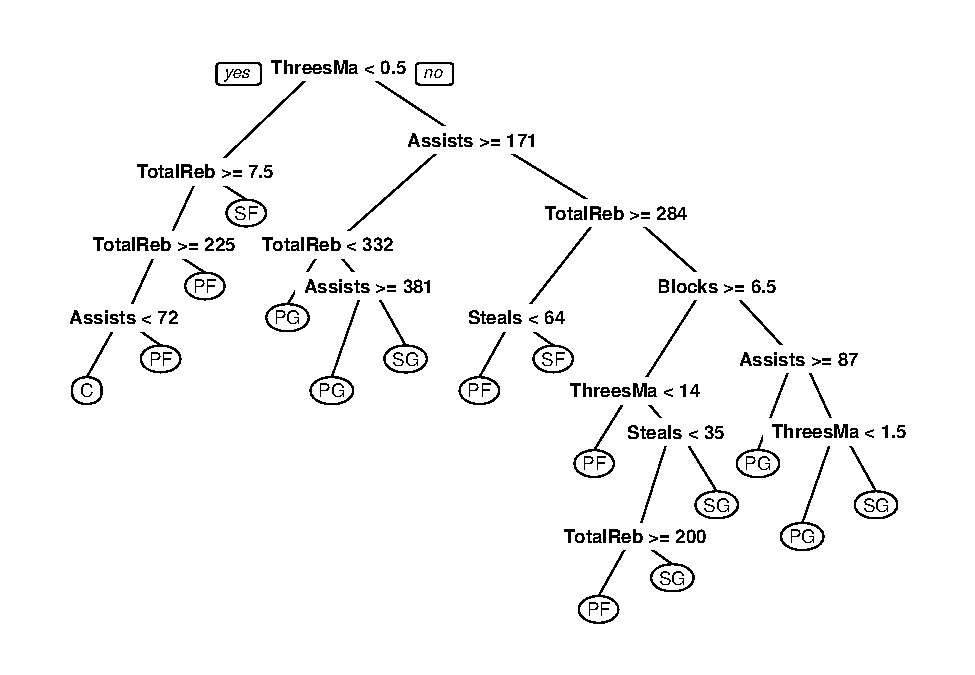
\includegraphics{DataAnalyticsWithR_files/figure-latex/unnamed-chunk-61-1.pdf}

阻攻/籃板/三分/助攻/抄截判斷位置-訓練

\begin{Shaded}
\begin{Highlighting}[]
\KeywordTok{prp}\NormalTok{(DT)}
\end{Highlighting}
\end{Shaded}

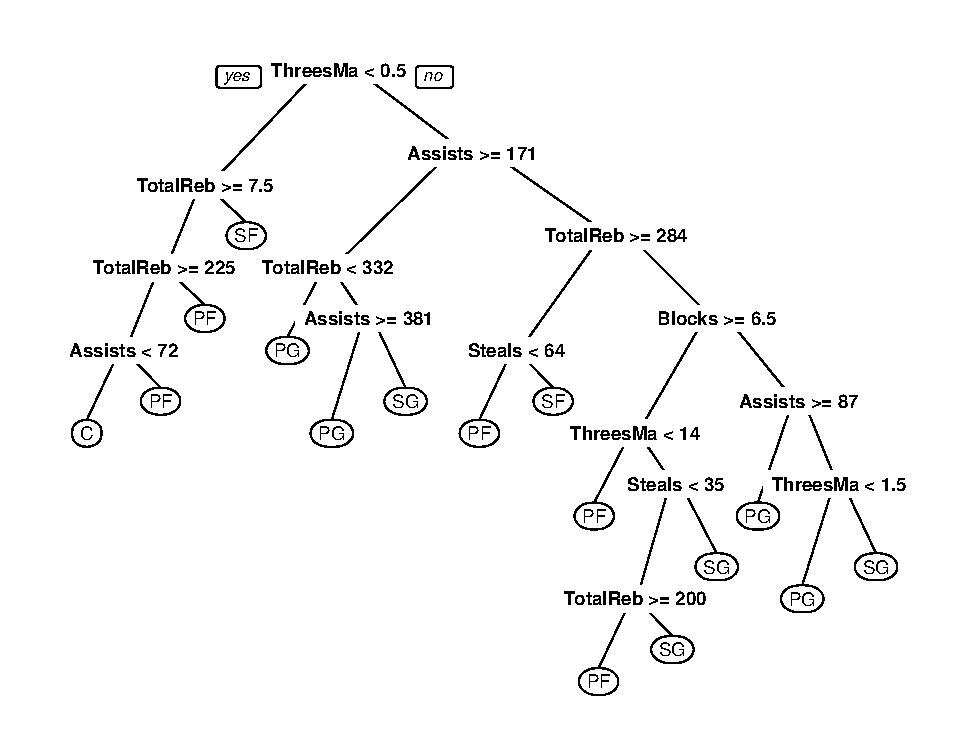
\includegraphics{DataAnalyticsWithR_files/figure-latex/unnamed-chunk-62-1.pdf}

有批球員沒寫守備位置?--預測

\begin{Shaded}
\begin{Highlighting}[]
\NormalTok{posPred<-}\KeywordTok{predict}\NormalTok{(DT,}\DataTypeTok{newdata=}\NormalTok{ NBA1516[NBA1516}\OperatorTok{$}\NormalTok{Test}\OperatorTok{==}\NormalTok{T,]) }\CommentTok{#Test==T, test data}
\CommentTok{# 預設為class probabilities, type = "prob"}
\KeywordTok{head}\NormalTok{(posPred)}
\end{Highlighting}
\end{Shaded}

\begin{verbatim}
##        C    PF   PG   SF   SG
## 1  0.167 0.083 0.00 0.75 0.00
## 2  0.000 0.000 0.67 0.00 0.33
## 10 0.025 0.075 0.20 0.22 0.47
## 11 0.000 0.120 0.04 0.36 0.48
## 13 0.357 0.643 0.00 0.00 0.00
## 14 0.029 0.000 0.15 0.15 0.68
\end{verbatim}

有個人沒寫守備位置--對答案

\begin{Shaded}
\begin{Highlighting}[]
\NormalTok{result<-}\KeywordTok{cbind}\NormalTok{(}\KeywordTok{round}\NormalTok{(posPred,}\DataTypeTok{digits =} \DecValTok{2}\NormalTok{),}
\NormalTok{              NBA1516[NBA1516}\OperatorTok{$}\NormalTok{Test}\OperatorTok{==}\NormalTok{T,]}\OperatorTok{$}\NormalTok{Name,}
      \KeywordTok{as.character}\NormalTok{(NBA1516[NBA1516}\OperatorTok{$}\NormalTok{Test}\OperatorTok{==}\NormalTok{T,]}\OperatorTok{$}\NormalTok{Position))}
\KeywordTok{head}\NormalTok{(result)}
\end{Highlighting}
\end{Shaded}

\begin{verbatim}
##    C      PF     PG     SF     SG                            
## 1  "0.17" "0.08" "0"    "0.75" "0"    "Jared Dudley"     "SG"
## 2  "0"    "0"    "0.67" "0"    "0.33" "Spence Dinwiddie" "PG"
## 10 "0.02" "0.08" "0.2"  "0.22" "0.48" "Doug Mcdermott"   "SF"
## 11 "0"    "0.12" "0.04" "0.36" "0.48" "James Johnson"    "PF"
## 13 "0.36" "0.64" "0"    "0"    "0"    "Joakim Noah"      "C" 
## 14 "0.03" "0"    "0.15" "0.15" "0.68" "Bradley Beal"     "SG"
\end{verbatim}

有個人沒寫守備位置--預測-2

\begin{Shaded}
\begin{Highlighting}[]
\NormalTok{posPredC<-}\KeywordTok{predict}\NormalTok{(DT,}\DataTypeTok{newdata=}\NormalTok{ NBA1516[NBA1516}\OperatorTok{$}\NormalTok{Test}\OperatorTok{==}\NormalTok{T,],}\DataTypeTok{type =} \StringTok{"class"}\NormalTok{)}
\CommentTok{# type = "class" 直接預測類別}
\KeywordTok{head}\NormalTok{(posPredC)}
\end{Highlighting}
\end{Shaded}

\begin{verbatim}
##  1  2 10 11 13 14 
## SF PG SG SG PF SG 
## Levels: C PF PG SF SG
\end{verbatim}

有個人沒寫守備位置--對答案-2

\begin{Shaded}
\begin{Highlighting}[]
\NormalTok{resultC<-}\KeywordTok{cbind}\NormalTok{(}\KeywordTok{as.character}\NormalTok{(posPredC),NBA1516[NBA1516}\OperatorTok{$}\NormalTok{Test}\OperatorTok{==}\NormalTok{T,]}\OperatorTok{$}\NormalTok{Name,}
      \KeywordTok{as.character}\NormalTok{(NBA1516[NBA1516}\OperatorTok{$}\NormalTok{Test}\OperatorTok{==}\NormalTok{T,]}\OperatorTok{$}\NormalTok{Position))}
\KeywordTok{head}\NormalTok{(resultC)}
\end{Highlighting}
\end{Shaded}

\begin{verbatim}
##      [,1] [,2]               [,3]
## [1,] "SF" "Jared Dudley"     "SG"
## [2,] "PG" "Spence Dinwiddie" "PG"
## [3,] "SG" "Doug Mcdermott"   "SF"
## [4,] "SG" "James Johnson"    "PF"
## [5,] "PF" "Joakim Noah"      "C" 
## [6,] "SG" "Bradley Beal"     "SG"
\end{verbatim}

\hypertarget{case-study}{%
\section{Case Study}\label{case-study}}

完整的模型建立步驟範例:

\begin{itemize}
\tightlist
\item
  標題:以聲波撞擊礦石的回聲預測礦石是否為礦物
\item
  以Sonar, Mines vs.~Rocks為例
\end{itemize}

\textbf{步驟1.1:讀資料}

\begin{Shaded}
\begin{Highlighting}[]
\CommentTok{#install.packages("mlbench") # 此package內有很多dataset可練習}
\KeywordTok{library}\NormalTok{(mlbench)}
\KeywordTok{data}\NormalTok{(Sonar)}
\KeywordTok{str}\NormalTok{(Sonar) }\CommentTok{#看一下資料型別,有沒有缺值,類別變項是不是factor}
\end{Highlighting}
\end{Shaded}

\begin{verbatim}
## 'data.frame':    208 obs. of  61 variables:
##  $ V1   : num  0.02 0.0453 0.0262 0.01 0.0762 0.0286 0.0317 0.0519 0.0223 0.0164 ...
##  $ V2   : num  0.0371 0.0523 0.0582 0.0171 0.0666 0.0453 0.0956 0.0548 0.0375 0.0173 ...
##  $ V3   : num  0.0428 0.0843 0.1099 0.0623 0.0481 ...
##  $ V4   : num  0.0207 0.0689 0.1083 0.0205 0.0394 ...
##  $ V5   : num  0.0954 0.1183 0.0974 0.0205 0.059 ...
##  $ V6   : num  0.0986 0.2583 0.228 0.0368 0.0649 ...
##  $ V7   : num  0.154 0.216 0.243 0.11 0.121 ...
##  $ V8   : num  0.16 0.348 0.377 0.128 0.247 ...
##  $ V9   : num  0.3109 0.3337 0.5598 0.0598 0.3564 ...
##  $ V10  : num  0.211 0.287 0.619 0.126 0.446 ...
##  $ V11  : num  0.1609 0.4918 0.6333 0.0881 0.4152 ...
##  $ V12  : num  0.158 0.655 0.706 0.199 0.395 ...
##  $ V13  : num  0.2238 0.6919 0.5544 0.0184 0.4256 ...
##  $ V14  : num  0.0645 0.7797 0.532 0.2261 0.4135 ...
##  $ V15  : num  0.066 0.746 0.648 0.173 0.453 ...
##  $ V16  : num  0.227 0.944 0.693 0.213 0.533 ...
##  $ V17  : num  0.31 1 0.6759 0.0693 0.7306 ...
##  $ V18  : num  0.3 0.887 0.755 0.228 0.619 ...
##  $ V19  : num  0.508 0.802 0.893 0.406 0.203 ...
##  $ V20  : num  0.48 0.782 0.862 0.397 0.464 ...
##  $ V21  : num  0.578 0.521 0.797 0.274 0.415 ...
##  $ V22  : num  0.507 0.405 0.674 0.369 0.429 ...
##  $ V23  : num  0.433 0.396 0.429 0.556 0.573 ...
##  $ V24  : num  0.555 0.391 0.365 0.485 0.54 ...
##  $ V25  : num  0.671 0.325 0.533 0.314 0.316 ...
##  $ V26  : num  0.641 0.32 0.241 0.533 0.229 ...
##  $ V27  : num  0.71 0.327 0.507 0.526 0.7 ...
##  $ V28  : num  0.808 0.277 0.853 0.252 1 ...
##  $ V29  : num  0.679 0.442 0.604 0.209 0.726 ...
##  $ V30  : num  0.386 0.203 0.851 0.356 0.472 ...
##  $ V31  : num  0.131 0.379 0.851 0.626 0.51 ...
##  $ V32  : num  0.26 0.295 0.504 0.734 0.546 ...
##  $ V33  : num  0.512 0.198 0.186 0.612 0.288 ...
##  $ V34  : num  0.7547 0.2341 0.2709 0.3497 0.0981 ...
##  $ V35  : num  0.854 0.131 0.423 0.395 0.195 ...
##  $ V36  : num  0.851 0.418 0.304 0.301 0.418 ...
##  $ V37  : num  0.669 0.384 0.612 0.541 0.46 ...
##  $ V38  : num  0.61 0.106 0.676 0.881 0.322 ...
##  $ V39  : num  0.494 0.184 0.537 0.986 0.283 ...
##  $ V40  : num  0.274 0.197 0.472 0.917 0.243 ...
##  $ V41  : num  0.051 0.167 0.465 0.612 0.198 ...
##  $ V42  : num  0.2834 0.0583 0.2587 0.5006 0.2444 ...
##  $ V43  : num  0.282 0.14 0.213 0.321 0.185 ...
##  $ V44  : num  0.4256 0.1628 0.2222 0.3202 0.0841 ...
##  $ V45  : num  0.2641 0.0621 0.2111 0.4295 0.0692 ...
##  $ V46  : num  0.1386 0.0203 0.0176 0.3654 0.0528 ...
##  $ V47  : num  0.1051 0.053 0.1348 0.2655 0.0357 ...
##  $ V48  : num  0.1343 0.0742 0.0744 0.1576 0.0085 ...
##  $ V49  : num  0.0383 0.0409 0.013 0.0681 0.023 0.0264 0.0507 0.0285 0.0777 0.0092 ...
##  $ V50  : num  0.0324 0.0061 0.0106 0.0294 0.0046 0.0081 0.0159 0.0178 0.0439 0.0198 ...
##  $ V51  : num  0.0232 0.0125 0.0033 0.0241 0.0156 0.0104 0.0195 0.0052 0.0061 0.0118 ...
##  $ V52  : num  0.0027 0.0084 0.0232 0.0121 0.0031 0.0045 0.0201 0.0081 0.0145 0.009 ...
##  $ V53  : num  0.0065 0.0089 0.0166 0.0036 0.0054 0.0014 0.0248 0.012 0.0128 0.0223 ...
##  $ V54  : num  0.0159 0.0048 0.0095 0.015 0.0105 0.0038 0.0131 0.0045 0.0145 0.0179 ...
##  $ V55  : num  0.0072 0.0094 0.018 0.0085 0.011 0.0013 0.007 0.0121 0.0058 0.0084 ...
##  $ V56  : num  0.0167 0.0191 0.0244 0.0073 0.0015 0.0089 0.0138 0.0097 0.0049 0.0068 ...
##  $ V57  : num  0.018 0.014 0.0316 0.005 0.0072 0.0057 0.0092 0.0085 0.0065 0.0032 ...
##  $ V58  : num  0.0084 0.0049 0.0164 0.0044 0.0048 0.0027 0.0143 0.0047 0.0093 0.0035 ...
##  $ V59  : num  0.009 0.0052 0.0095 0.004 0.0107 0.0051 0.0036 0.0048 0.0059 0.0056 ...
##  $ V60  : num  0.0032 0.0044 0.0078 0.0117 0.0094 0.0062 0.0103 0.0053 0.0022 0.004 ...
##  $ Class: Factor w/ 2 levels "M","R": 2 2 2 2 2 2 2 2 2 2 ...
\end{verbatim}

在建立模型之前\ldots 別忘了基本的資料分析,使用\texttt{探索性分析\ Exploratory\ data\ analysis},看看資料長怎麼樣,要是有一個參數可以完美的把礦物跟石頭分開,那就不用麻煩建模了\ldots{}

探索性分析 Exploratory data analysis

\begin{Shaded}
\begin{Highlighting}[]
\KeywordTok{library}\NormalTok{(ggplot2);}\KeywordTok{library}\NormalTok{(reshape2) }\CommentTok{#install.packages(c("ggplot2","reshape2"))}
\NormalTok{Sonar.m<-}\KeywordTok{melt}\NormalTok{(Sonar,}\DataTypeTok{id.vars =} \KeywordTok{c}\NormalTok{(}\StringTok{"Class"}\NormalTok{))}
\KeywordTok{ggplot}\NormalTok{(Sonar.m)}\OperatorTok{+}\KeywordTok{geom_boxplot}\NormalTok{(}\KeywordTok{aes}\NormalTok{(}\DataTypeTok{x=}\NormalTok{Class,}\DataTypeTok{y=}\NormalTok{value))}\OperatorTok{+}
\StringTok{    }\KeywordTok{facet_wrap}\NormalTok{(}\OperatorTok{~}\NormalTok{variable, }\DataTypeTok{nrow=}\DecValTok{5}\NormalTok{,}\DataTypeTok{scales =} \StringTok{"free_y"}\NormalTok{) }\CommentTok{#圖片太小了}
\end{Highlighting}
\end{Shaded}

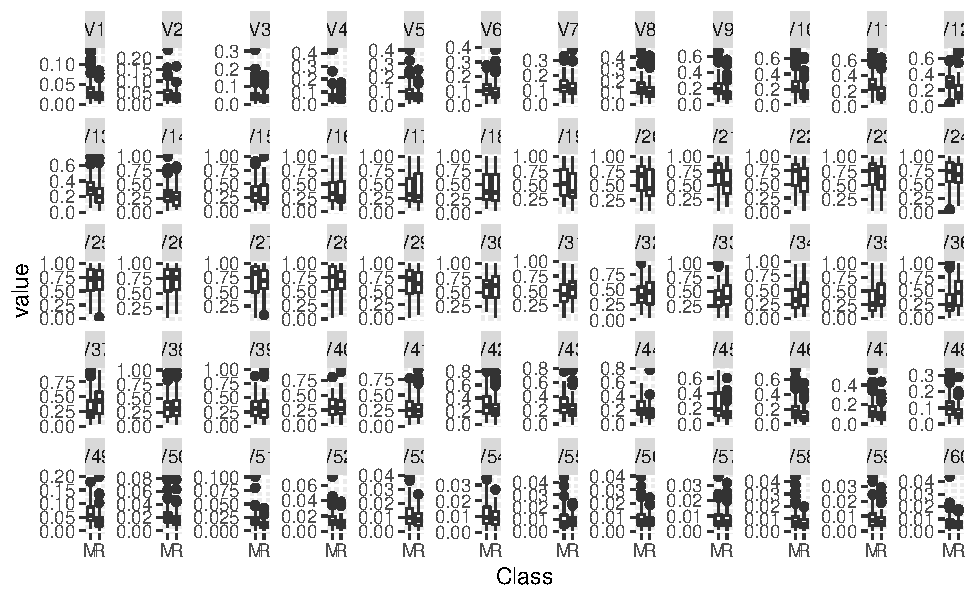
\includegraphics{DataAnalyticsWithR_files/figure-latex/unnamed-chunk-68-1.pdf}

\textbf{步驟1.2: 資料前處理}

\begin{itemize}
\tightlist
\item
  缺值?

  \begin{itemize}
  \tightlist
  \item
    沒有缺值,不需要處理
  \end{itemize}
\item
  答案種類?

  \begin{itemize}
  \tightlist
  \item
    類別變項叫\texttt{Class},M: mine礦--\textgreater+, R: rock--\textgreater-,不需要處理
  \end{itemize}
\item
  類別變項的型別是不是factor?

  \begin{itemize}
  \tightlist
  \item
    是,不需要處理
  \end{itemize}
\item
  有沒有無關的參數?

  \begin{itemize}
  \tightlist
  \item
    沒有無關的參數,不需要處理
  \end{itemize}
\end{itemize}

\textbf{步驟2:分成訓練組與測試組}

該怎麼分可以自己決定,1/3,1/5\ldots 都可以

\begin{Shaded}
\begin{Highlighting}[]
\NormalTok{Sonar}\OperatorTok{$}\NormalTok{Test<-F }\CommentTok{#新增一個參數紀錄分組}
\CommentTok{#隨機取1/3當Test set}
\NormalTok{Sonar[}\KeywordTok{sample}\NormalTok{(}\DecValTok{1}\OperatorTok{:}\KeywordTok{nrow}\NormalTok{(Sonar),}\KeywordTok{nrow}\NormalTok{(Sonar)}\OperatorTok{/}\DecValTok{3}\NormalTok{),]}\OperatorTok{$}\NormalTok{Test<-T}
\CommentTok{# 看一下 Training set : Test set 案例數}
\KeywordTok{c}\NormalTok{(}\KeywordTok{sum}\NormalTok{(Sonar}\OperatorTok{$}\NormalTok{Test}\OperatorTok{==}\NormalTok{F),}\KeywordTok{sum}\NormalTok{(Sonar}\OperatorTok{$}\NormalTok{Test}\OperatorTok{==}\NormalTok{T))}
\end{Highlighting}
\end{Shaded}

\begin{verbatim}
## [1] 139  69
\end{verbatim}

\textbf{步驟3:訓練模型}

\begin{itemize}
\tightlist
\item
  注意只能用\texttt{訓練組}的資料,\texttt{Test}參數==F,忘記可以看前面範例
\item
  數值自變項X很多,先用迴歸好了~
\item
  要解釋一下模型
\end{itemize}

\begin{Shaded}
\begin{Highlighting}[]
\NormalTok{fit<-}\KeywordTok{glm}\NormalTok{(Class}\OperatorTok{~}\NormalTok{., Sonar[Sonar}\OperatorTok{$}\NormalTok{Test}\OperatorTok{==}\NormalTok{F,],}\DataTypeTok{family=}\StringTok{"binomial"}\NormalTok{)}
\NormalTok{finalFit<-}\KeywordTok{stepAIC}\NormalTok{(fit,}\DataTypeTok{direction =} \StringTok{"both"}\NormalTok{,}\DataTypeTok{trace =}\NormalTok{ F)}
\KeywordTok{summary}\NormalTok{(finalFit)}\OperatorTok{$}\NormalTok{coefficients}
\end{Highlighting}
\end{Shaded}

\begin{verbatim}
##             Estimate Std. Error z value Pr(>|z|)
## (Intercept)     1975     123555  0.0160     0.99
## V1            -36138    1993240 -0.0181     0.99
## V3              6804     564355  0.0121     0.99
## V7              1529     448633  0.0034     1.00
## V13            -7142     400539 -0.0178     0.99
## V16             4645     288291  0.0161     0.99
## V20            -2894     166553 -0.0174     0.99
## V21             3240     210433  0.0154     0.99
## V22            -3376     214501 -0.0157     0.99
## V29             3485     237301  0.0147     0.99
## V30            -8290     483660 -0.0171     0.99
## V31             9150     486567  0.0188     0.98
## V32            -3974     254600 -0.0156     0.99
## V34             2526     144907  0.0174     0.99
## V35            -4344     241713 -0.0180     0.99
## V36             5142     281220  0.0183     0.99
## V38            -3674     202378 -0.0182     0.99
## V39             3541     211325  0.0168     0.99
## V47            -4577     326253 -0.0140     0.99
## V49           -26603    1476038 -0.0180     0.99
## V50            43675    3120364  0.0140     0.99
## V55            35354    3125428  0.0113     0.99
\end{verbatim}

\textbf{步驟4.1:用測試組驗證模型-預測}

\begin{Shaded}
\begin{Highlighting}[]
\NormalTok{MinePred<-}\KeywordTok{predict}\NormalTok{(finalFit,}\DataTypeTok{newdata =}\NormalTok{ Sonar[Sonar}\OperatorTok{$}\NormalTok{Test}\OperatorTok{==}\NormalTok{T,])}
\NormalTok{MineAns<-}\KeywordTok{ifelse}\NormalTok{(MinePred}\OperatorTok{<}\FloatTok{0.5}\NormalTok{,}\StringTok{"M"}\NormalTok{,}\StringTok{"R"}\NormalTok{) }\CommentTok{#<0.5: Level 1}
\NormalTok{MineAns<-}\KeywordTok{factor}\NormalTok{(MineAns,}\DataTypeTok{levels =} \KeywordTok{c}\NormalTok{(}\StringTok{"M"}\NormalTok{,}\StringTok{"R"}\NormalTok{))}
\NormalTok{MineAns}
\end{Highlighting}
\end{Shaded}

\begin{verbatim}
##   9  32  38  41  43  45  49  54  55  59  60  65  66  68  69  72  75  80 
##   M   M   M   M   M   M   R   M   M   M   M   R   M   R   R   M   R   R 
##  83  84  86  88  90  91  92  95  96  98 100 106 107 110 111 115 117 119 
##   M   M   M   R   M   R   M   R   R   R   R   M   R   R   M   M   R   R 
## 128 129 131 132 133 135 137 139 144 148 150 153 154 156 157 159 160 167 
##   R   M   R   R   R   M   R   R   R   R   M   M   R   M   M   M   R   M 
## 169 171 172 173 174 177 179 187 189 191 193 194 196 201 208 
##   R   M   R   R   R   M   M   M   M   R   M   M   R   R   M 
## Levels: M R
\end{verbatim}

\textbf{步驟4.2:用測試組驗證模型-效能}

\begin{Shaded}
\begin{Highlighting}[]
\KeywordTok{library}\NormalTok{(caret) }\CommentTok{# install.packages("caret") #計算參數的packages}
\KeywordTok{sensitivity}\NormalTok{(MineAns,Sonar[Sonar}\OperatorTok{$}\NormalTok{Test}\OperatorTok{==}\NormalTok{T,]}\OperatorTok{$}\NormalTok{Class)}
\end{Highlighting}
\end{Shaded}

\begin{verbatim}
## [1] 0.87
\end{verbatim}

\begin{Shaded}
\begin{Highlighting}[]
\KeywordTok{specificity}\NormalTok{(MineAns,Sonar[Sonar}\OperatorTok{$}\NormalTok{Test}\OperatorTok{==}\NormalTok{T,]}\OperatorTok{$}\NormalTok{Class)}
\end{Highlighting}
\end{Shaded}

\begin{verbatim}
## [1] 0.93
\end{verbatim}

\begin{Shaded}
\begin{Highlighting}[]
\KeywordTok{posPredValue}\NormalTok{(MineAns,Sonar[Sonar}\OperatorTok{$}\NormalTok{Test}\OperatorTok{==}\NormalTok{T,]}\OperatorTok{$}\NormalTok{Class)}
\end{Highlighting}
\end{Shaded}

\begin{verbatim}
## [1] 0.94
\end{verbatim}

\begin{Shaded}
\begin{Highlighting}[]
\KeywordTok{negPredValue}\NormalTok{(MineAns,Sonar[Sonar}\OperatorTok{$}\NormalTok{Test}\OperatorTok{==}\NormalTok{T,]}\OperatorTok{$}\NormalTok{Class)}
\end{Highlighting}
\end{Shaded}

\begin{verbatim}
## [1] 0.85
\end{verbatim}

\textbf{解釋範例 - 資料說明}

此資料來源為UCI Machine Learning Repository。

記載礦物與石頭接受各個不同角度的聲波撞擊後,接收到的回聲數值,一共有60個參數,代表使用一特別角度的聲波撞擊礦石所得回聲。另外,分類結果為二元分類,包括礦物 (M) 與石頭 (R) 。

\textbf{解釋範例 - 模型說明}

使用聲波在不同角度撞擊\texttt{礦石}所得到的回聲資料,以邏輯迴歸建立模型預測礦石是否為礦物,經最佳化後,模型使用參數為V1 + V2 + V3 + V4 + V7 + V11 + V12 + V13 + V17 + V18 + V22 + V24 + V25 + V26 + V30 + V31 + V32 + V38 + V39 + V48 + V50 + V52 + V53 + V58 + V59,共25個參數,各參數代表從一特別角度所得的礦石回聲

\textbf{解釋範例 - 預測效能說明}

使用聲波在不同角度撞擊\texttt{礦石}所得到的回聲資料,以邏輯迴歸模型預測礦石是否為礦物,可得敏感度97\%,特異性89\%,陽性預測率89\%,陰性預測率97\%。

\hypertarget{ux53c3ux8003ux8cc7ux6599-1}{%
\section{參考資料}\label{ux53c3ux8003ux8cc7ux6599-1}}

\begin{itemize}
\item
  台大資工林軒田教授:

  \begin{itemize}
  \tightlist
  \item
    \href{www.coursera.org/course/ntumlone}{Machine Learning Foundations}
  \item
    \href{www.coursera.org/course/ntumltwo}{Machine Learning Techniques}
  \end{itemize}
\item
  \href{http://www.salemmarafi.com/code/market-basket-analysis-with-r/}{Market Basket Analysis with R}
\item
  \href{https://www.r-bloggers.com/deep-learning-in-r-2/}{Deep Learning in R}
\end{itemize}

\hypertarget{big}{%
\chapter{從小數據到大數據分析}\label{big}}

Placeholder

\hypertarget{r-hadoop}{%
\section{R + Hadoop}\label{r-hadoop}}

\hypertarget{rhadoopux5b89ux88ddux6e2cux8a66ux6d41ux7a0b-cloudera}{%
\section{RHadoop安裝測試流程 (Cloudera)}\label{rhadoopux5b89ux88ddux6e2cux8a66ux6d41ux7a0b-cloudera}}

\hypertarget{ux7cfbux7d71ux8edfux9ad4ux7248ux672cux8cc7ux8a0a}{%
\subsection{系統/軟體版本資訊}\label{ux7cfbux7d71ux8edfux9ad4ux7248ux672cux8cc7ux8a0a}}

\hypertarget{ux53c3ux8003ux8cc7ux6599-2}{%
\subsection{參考資料}\label{ux53c3ux8003ux8cc7ux6599-2}}

\hypertarget{ux5b89ux88ddux6b65ux9a5f}{%
\subsection{安裝步驟}\label{ux5b89ux88ddux6b65ux9a5f}}

\hypertarget{cloudera-cdh-quickstart-vm}{%
\subsubsection{Cloudera CDH QuickStart VM}\label{cloudera-cdh-quickstart-vm}}

\hypertarget{ux5b89ux88ddr}{%
\subsubsection{安裝R}\label{ux5b89ux88ddr}}

\hypertarget{ux5b89ux88ddrhadoop-1-ux5148ux9032ux884cux74b0ux5883ux8a2dux5b9a}{%
\subsubsection{安裝RHadoop-1 先進行環境設定}\label{ux5b89ux88ddrhadoop-1-ux5148ux9032ux884cux74b0ux5883ux8a2dux5b9a}}

\hypertarget{ux5b89ux88ddrhadoop-2-rmr2}{%
\subsubsection{安裝RHadoop-2 rmr2}\label{ux5b89ux88ddrhadoop-2-rmr2}}

\hypertarget{ux5b89ux88ddrhadoop-3-rhdfs}{%
\subsubsection{安裝RHadoop-3 rhdfs}\label{ux5b89ux88ddrhadoop-3-rhdfs}}

\hypertarget{ux6e2cux8a66ux524dux5148ux89e3ux6c7aux6b0aux9650ux554fux984c}{%
\subsection{測試前,先解決權限問題}\label{ux6e2cux8a66ux524dux5148ux89e3ux6c7aux6b0aux9650ux554fux984c}}

\hypertarget{ux6e2cux8a66}{%
\subsection{測試}\label{ux6e2cux8a66}}

\hypertarget{ux5b89ux88ddrstudio-server}{%
\subsection{安裝RStudio Server}\label{ux5b89ux88ddrstudio-server}}

\hypertarget{rhadoop-mapreduce-easy-word-count}{%
\section{RHadoop MapReduce: easy word count}\label{rhadoop-mapreduce-easy-word-count}}

\hypertarget{r-spark}{%
\section{R + Spark}\label{r-spark}}

\hypertarget{install}{%
\chapter{軟體安裝介紹}\label{install}}

Placeholder

\hypertarget{rux5b89ux88dd}{%
\section{R安裝}\label{rux5b89ux88dd}}

\hypertarget{rstudioux5b89ux88dd}{%
\section{RStudio安裝}\label{rstudioux5b89ux88dd}}

\hypertarget{rstudioux4f7fux7528ux7c21ux4ecb}{%
\section{RStudio使用簡介}\label{rstudioux4f7fux7528ux7c21ux4ecb}}

\hypertarget{ux5c08ux6848}{%
\subsection{專案}\label{ux5c08ux6848}}

\hypertarget{rstudioux4ecbux9762}{%
\subsection{RStudio介面}\label{rstudioux4ecbux9762}}

\hypertarget{author}{%
\chapter*{作者資訊}\label{author}}
\addcontentsline{toc}{chapter}{作者資訊}

曾意儒 Yi-Ju Tseng

\href{http://im.cgu.edu.tw/bin/home.php}{長庚大學 資訊管理學系} 助理教授

\href{http://yijutseng.github.io}{個人網站}

Lab: \href{https://dhlab-cgu.github.io/}{數位健康實驗室}

歡迎提供\href{https://goo.gl/forms/5Htobvwy2vsB7yiF3}{建議與回饋}

\bibliography{book.bib,packages.bib}


\end{document}
